\documentclass[12pt,a4paper]{report}
\usepackage[utf8]{inputenc}
\usepackage[spanish]{babel}
\usepackage[T1]{fontenc}
\usepackage{graphicx}
\usepackage{hyperref}
\usepackage{apacite} % debe ir después de hyperref







\usepackage[usenames, dvipsnames]{color}

%adjust your page margins here
\usepackage[top=0.70in, bottom=0.70in, left=0.8in,right=0.80in]{geometry} % setting the page alignment with this package
\usepackage[pdftex]{graphicx} %for embedding images
\usepackage[%dvips, % commented for pdflatex
bookmarks,  colorlinks=false]{hyperref} %for creating links in the pdf version and other additional pdf attributes, no effect on the printed document
\hypersetup{%
    pdfborder = {0 0 0}
}
\usepackage[final]{pdfpages} %for embedding another pdf, remove if not required
\usepackage{float} %used for figure placement with H as a parameter
\usepackage{hyperref}

%% Paquete para referencias de APA
%% Importante: Debe incluirse después de hyperref
\usepackage[]{apacite}

\usepackage{pslatex} % for times new roman, old package, but works
\usepackage{array} % for making text bold in table
\usepackage{setspace}
\usepackage{float}
\usepackage{enumerate}
\usepackage{longtable}
\usepackage{amssymb}
\usepackage[skip=2pt]{caption} % en el preámbulo


\usepackage[font=small,labelfont=bf]{caption}
\def\figurename{\textbf{Figure }}

\usepackage{listings}

\definecolor{dkgreen}{rgb}{0,0.6,0}
\definecolor{gray}{rgb}{0.5,0.5,0.5}
\definecolor{mauve}{rgb}{0.58,0,0.82}
 
\lstset{ %
  language=Java,                % the language of the code
  basicstyle=\footnotesize,           % the size of the fonts that are used for the code
  numbers=left,                   % where to put the line-numbers
  numberstyle=\tiny\color{gray},  % the style that is used for the line-numbers
  stepnumber=1,                   % each line is numbered
  numbersep=5pt,                  % how far the line-numbers are from the code
  backgroundcolor=\color{white},      % choose the background color. You must add \usepackage{color}
  showspaces=false,               % show spaces adding particular underscores
  showstringspaces=false,         % underline spaces within strings
  showtabs=false,                 % show tabs within strings adding particular underscores
  frame=single,                   % adds a frame around the code
  rulecolor=\color{black},        % if not set, the frame-color may be changed on line-breaks within not-black text (e.g. commens (green here))
  tabsize=2,                      % sets default tabsize to 2 spaces
  captionpos=b,                   % sets the caption-position to bottom
  breaklines=true,                % sets automatic line breaking
  breakatwhitespace=false,        % sets if automatic breaks should only happen at whitespace
  title=\lstname,                   % show the filename of files included with \lstinputlisting;
                                  % also try caption instead of title
  keywordstyle=\color{blue},          % keyword style
  commentstyle=\color{dkgreen},       % comment style
  stringstyle=\color{mauve},         % string literal style
  escapeinside={\%*}{*)},            % if you want to add a comment within your code
  morekeywords={*,...}               % if you want to add more keywords to the set
}

%For the header and footer
\usepackage{fancyhdr}
\fancypagestyle{plain}{%
\fancyfoot[L]{\emph{TEC, Unidad de Ingeniería en Computación de San José}} % except the center
\fancyfoot[R]{\thepage}
\renewcommand{\headrulewidth}{0.4pt}
\renewcommand{\footrulewidth}{0.4pt}
}

\pagestyle{fancy}

\rhead{\emph{Komuness}}

%\fancyfoot[LO,L]{\emph{Ingeniería en Computación, ITCR}}
\cfoot{}
\fancyfoot[RO, R]{\thepage}
\renewcommand{\headrulewidth}{0.4pt}
\renewcommand{\footrulewidth}{0.4pt}
%For the header and footer Over

%Page Border
\usepackage{pgf}
\usepackage{pgfpages}

\pgfpagesdeclarelayout{boxed}
{
  \edef\pgfpageoptionborder{0pt}
}
{
  \pgfpagesphysicalpageoptions
  {%
    logical pages=1,%
  }
  \pgfpageslogicalpageoptions{1}
  {
    border code=\pgfsetlinewidth{2pt}\pgfstroke,%
    border shrink=\pgfpageoptionborder,%
    resized width=.95\pgfphysicalwidth,%
    resized height=.95\pgfphysicalheight,%
    center=\pgfpoint{.5\pgfphysicalwidth}{.5\pgfphysicalheight}%
  }%
}
\pgfpagesuselayout{boxed}
\setlength{\parindent}{1cm}
%GLOBAL SETTINGS OVER, DOCUMENT BEGINS
\usepackage{tikz}
\usepackage{amsmath}

\usetikzlibrary{positioning, shapes.geometric, arrows, arrows.meta}
\begin{document}
\renewcommand\bibname{Referencias bibliográficas}
\lhead{ }

%FROM HERE YOUR PAGES START GETTING ADDED

% includes the cover page
\newpage
\begin{center}
\thispagestyle{empty}

\includegraphics[scale=1]{project/images/Firma-TEC.png}\\
\vspace{1cm}
\Large{\textbf{INFORME DE AVANCE DEL SPRINT 1\\ \large{DEL PROYECTO}}}\\[1cm]
\LARGE{\textsc {\textbf{``Sistema comunitario para jóvenes de la zona de
 Tejarcillos de Alajuelita''}}}\\[3cm]
\Large{\textbf{\\Para el curso de}}
\LARGE{\textbf{\\PROYECTO DE INGENIERÍA DE SOFTWARE\\}}
\vspace{0.5cm}
\vspace{1cm}
\Large{\textbf{\\EQUIPO DE TRABAJO}}\\[0.3cm]
\begin{table}[h]
\centering
\large{
\begin{tabular}{>{\bfseries}lc>{\bfseries}r}
Angélica Díaz Barrios & & Desarrolladora\\ %SCRUM MASTER
Fredrik Aburto Jiménez & & Desarrollador\\
Andrés Salas Araya & & Desarrollador\\

 & & \\
\end{tabular}}
\end{table}
\vspace{0.5cm}
\large{\textbf{BAJO LA SUPERVISIÓN DE}}\\
\large{\textbf{RODOLFO MORA ZAMORA}}\\
\vspace{1cm}
\large{\textbf{SAN JOSÉ}}
\large{\textbf{\\2025}}\\
\vspace{1cm}
\newpage
\end{center}
\newpage

\begin{center}
\thispagestyle{empty}
\vspace{2cm}
\LARGE{\textbf{RESUMEN}}\\[1.0cm]
\end{center}
\thispagestyle{empty}
Este documento presenta el informe del Sprint 1 del proyecto de plataforma digital para la comunidad de Tejarcillos, Alajuelita, promovido por Komuness CR (organización derivada de Coopesinergía). Este primer producto mínimo viable (MVP) se enfoca en reducir la brecha social y tecnológica mediante la entrega de una plataforma estable y funcional que permita a jóvenes y vecinos visibilizar sus talentos, productos y servicios culturales.

El Sprint 1 aborda la continuación del desarrollo parcial existente, mejorando significativamente la estabilidad del sistema, corrigiendo fallos críticos y optimizando la usabilidad. Las funcionalidades implementadas en esta iteración incluyen: sistema de categorización de contenidos, calendario interactivo de eventos, servidor confiable para almacenamiento de archivos, y correcciones integrales en los módulos de publicaciones y biblioteca digital.

Este primer MVP establece las bases tecnológicas sólidas para las futuras iteraciones que incorporarán roles de usuario, perfiles públicos, banco de profesionales y sistema de membresías premium. La iniciativa busca fortalecer el empoderamiento juvenil, la inclusión tecnológica y la participación cultural, consolidándose como un recurso duradero para la comunidad, con una plataforma probada y estable desde su primera versión funcional. % adds the abstract page
\newpage

%TABLE OF CONTENTS AND LIST OF FIGURES ARE AUTOMATICALLY ADDED BY FOLLOWING COMMANDS
%ADD FIGURE OF TABLES IF YOU NEED TO, CHECK DOCUMENTATION
\pagenumbering{roman} %numbering before main content starts


%To reset the Header & Footer for TOC and LOF
\pagestyle{empty}
\addtocontents{toc}{\protect\thispagestyle{empty}}
\tableofcontents % adds Index Page

\addtocontents{lof}{\protect\thispagestyle{empty}}
\listoffigures % adds List of Figures
\cleardoublepage

%And reset back the settings we choose for Header and Footer
\pagestyle{fancy}

\newpage
\pagenumbering{arabic} %reset numbering to normal for the main content

\chapter{Anteproyecto}

\section{Descripción y Alcance del proyecto}
\subsection{Antecedentes}
El proyecto es solicitado por Komuness CR, una organización comunitaria dedicada a promover proyectos que fortalezcan el desarrollo social, cultural y educativo en comunidades en situación de vulnerabilidad, como el barrio de Tejarcillos en Alajuelita. Komuness CR se integró a la estructura de Coopesinergía, una cooperativa autogestionaria que realiza proyectos orientados al desarrollo humano integral, principalmente en comunidades con menor acceso a recursos básicos (P. Monge, comunicación personal, 18 de agosto de 2025).

La necesidad que motiva este proyecto es la marcada brecha social y tecnológica que limita las oportunidades de desarrollo de los habitantes de Tejarcillos, especialmente de los jóvenes. Esta población carece de espacios y recursos adecuados para exponer sus talentos, productos y servicios, lo que reduce su participación en actividades culturales, educativas y económicas (P. Monge y T. Chaverry, comunicación personal, 18 de agosto de 2025).

El proyecto solventará esta necesidad mediante el desarrollo de una plataforma digital que servirá como espacio para que los jóvenes y vecinos de Tejarcillos puedan compartir sus productos, servicios y eventos culturales, además de contar con una biblioteca digital donde se registren proyectos y materiales de interés. El impacto esperado es el fortalecimiento del empoderamiento juvenil, la inclusión tecnológica y la participación cultural.

Los beneficios del proyecto alcanzarán principalmente a los jóvenes y habitantes del barrio Tejarcillos en Alajuelita, cuyo estilo de vida podrá mejorar al contar con herramientas digitales que fomenten la inclusión y la equidad, brindando espacios para visibilizar y registrar proyectos culturales y comunitarios.

\subsection{Objetivos}

%
% Los objetivos del proyecto deben englobar el alcance total. Todo objetivo debe estar redactado respetando la siguiente estructura:

% Verbo infinitivo: Representa una acción que el equipo de desarrollo ejecutará durante el proyecto. Debe ser una acción concreta y relevante para completar el proyecto

% Objeto: Indica el objeto sobre el cual se aplicará la acción. Típicamente representa el producto esperado de la acción

% Modo: Indica parámetros por los cuales se medirá la calidad y completitud del resultado. 

% Ejemplo: Desarrollar un sistema de facturación electrónica que provea una interfaz amigable para el usuario y cumpla con los estándares impuestos por el Ministerio de Hacienda de Costa Rica. 

% Sólo puede existir un verbo infinitivo en el objetivo
% Debe ser posible medir el nivel de cumplimiento del objetivo, es decir, debe ser posible decir en cualquier momento del proyecto, cual porcentaje del objetivo se ha cumplido.

\begin{itemize}
    \item \textbf{Objetivo General}
    \begin{itemize}
        \item Desarrollar una plataforma digital para la comunidad juvenil de Alajuelita que visibilice sus talentos y servicios culturales mediante una biblioteca digital, mejore el sistema de publicaciones y garantice su sostenibilidad con un sistema de membresías premium, utilizando el stack tecnológico MERN e integrando APIs de PayPal para transacciones seguras.

    \end{itemize}
    \item \textbf{Objetivos Específicos}
    \begin{itemize}
        \item Optimizar el módulo de publicaciones y eventos de la plataforma que facilite la consulta y gestión de la información comunitaria, implementando un sistema de categorías, un calendario interactivo y un servidor para archivos.
         \item Integrar un sistema de usuarios premium y pagos mediante PayPal que permita la monetización de membresías, configurando límites de publicaciones y flujos de transacción.
        \item Integrar perfiles públicos y un banco de profesionales que facilite la búsqueda de talentos que forman parte de la comunidad.
    \end{itemize}
\end{itemize}

\subsection{Involucrados}
% Liste los diferentes involucrados en este proyecto, incluya en una figura un organigrama en el cual se ilustre la relación entre todos los participantes e interesados con los miembros del equipo de trabajo.

\begin{table}[H]
\caption{Involucrados en el proyecto}
\label{tab:involucrados}
\centering
\small
\begin{tabular}{|l|l|l|}
\hline
\textbf{Nombre del involucrado} & \textbf{Rol} & \textbf{Contacto} \\
\hline \hline
Rodolfo Mora Zamora & Supervisor - Profesor TEC & rodmora@itcr.ac.cr \\
\hline
Paola Monge & Cliente - Directora Fondo Inés Revueltas & komunesscr@gmail.com \\
\hline
Tatiana Chaverry & Cliente - Coordinadora Grupo Jóvenes Komuness & komunesscr@gmail.com \\
\hline
Fredrik Aburto Jiménez & Desarrollador - TEC & fredrik@estudiantec.cr \\
\hline
Angélica Díaz Barrios & Desarrolladora - TEC & diazbarrios2001@estudiantec.cr \\
\hline
Andrés Salas Araya & Desarrollador - TEC & asaraya153@estudiantec.cr \\
\hline
\end{tabular}
\caption{Lista de involucrados y sus contactos}
\end{table}

% Organigrama
\begin{figure}[H]
  \centering
  \begin{tikzpicture}[
      node distance=1.5cm and 2cm,
      every node/.style={rectangle, rounded corners, draw, align=center, minimum width=3cm, fill=blue!10},
      arrow/.style={->, thick, >=stealth}
    ]
    
    % Nodo supervisor
    \node (supervisor) [fill=red!20] {Supervisor\\Rodolfo Mora Zamora\\\small{Profesor TEC}};
    
    % Nodo cliente
    \node (cliente) [right=of supervisor, fill=green!20] {Cliente\\Komuness CR\\\small{P. Monge - T. Chaverry}};
    
    % Equipo de desarrollo
    \node (equipo) [below=2cm of supervisor, fill=yellow!20] {Equipo de Desarrollo\\Tecnológico de Costa Rica};
    
    % Desarrolladores
    \node (dev1) [below left=of equipo] {Fredrik Aburto Jiménez\\\small{Desarrollador}};
    \node (dev2) [below=of equipo] {Angélica Díaz Barrios\\\small{Desarrolladora}};
    \node (dev3) [below right=of equipo] {Andrés Salas Araya\\\small{Desarrollador}};
    
    % Líneas de conexión
    \draw[arrow] (supervisor) -- (equipo);
    \draw[arrow] (cliente) -- (equipo);
    \draw[arrow] (equipo) -- (dev1);
    \draw[arrow] (equipo) -- (dev2);
    \draw[arrow] (equipo) -- (dev3);
    
    % Línea de supervisión cliente
    \draw[dashed, arrow] (supervisor) to [bend left=15] (cliente);
    
  \end{tikzpicture}
  \caption{Organigrama de la estructura del equipo e involucrados del proyecto}
  \label{fig:organigrama}
\end{figure}

\subsection{Estructura de Desglose de Trabajo}

%Divida su proyecto en cuatro Productos Mínimos Viables (MVP por sus siglas en inglés),  cada MVP debe descomponerlo en entregables que deberá presentar a su cliente al final de cada iteración. Describa cada MVP en esta sección, indicando en cuáles subproductos se divide.

%Diagrame sus entregables en una Estructura de Desglose de Trabajo (EDT) que le facilite llevar un registro de cuáles se deben cumplir en cada etapa del proyecto. Utilice esta guía para orientarse en cómo desarrollar su EDT: https://formulaproyectosurbanospmipe.wordpress.com/2012/05/09/tema-n-5-la-estructura-de-desglose-del-trabajo-edt-segun-la-guia-del-pmbok-30-04-2012-sesion-10-segunda-parte/.

% EDT
\begin{figure}[H]
  \centering
    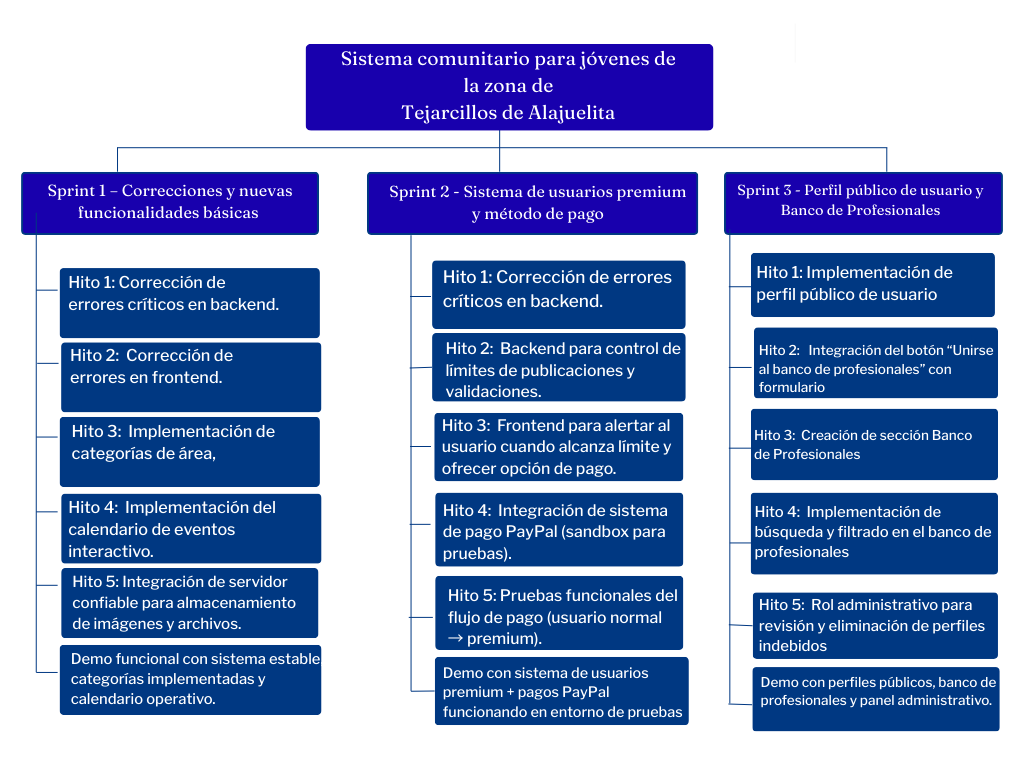
\includegraphics[height= 10cm, width=15cm]{project/images/EDT1.png}
  \caption{\textbf{Diagrama del alcance del proyecto dividido en sprints}}
\end{figure}
 % adds the introduction page
\chapter{Especificación de requerimientos}
\section{Pila de producto}
La plataforma digital para la comunidad de Tejarcillos se ha estructurado mediante un análisis detallado de historias de usuario que permiten visualizar en este informe el MVP 1 del sistema. Para facilitar la trazabilidad y comprensión de la estructura del sistema, se ha implementado una codificación RFXXX (Requerimiento Funcional) para todas las funcionalidades del producto y RNFXXX (Requerimiento No Funcional) para otros requerimientos.

Esta codificación unificada permite mantener una nomenclatura consistente para todos los requerimientos funcionales del sistema, facilitando su identificación, priorización y seguimiento throughout el desarrollo del proyecto.
\subsection{Requerimientos funcionales del sistema}

%% PILA DE PRODUCTO %%
\begin{longtable}{|l||p{7cm}|l|l|}
\multicolumn{4}{c}{Pila general del producto}\\
\hline\hline
\textbf{Código} & \textbf{Descripción} & \textbf{Prioridad} & \textbf{Inserción}\\
\hline
\endfirsthead
\textbf{Código} & \textbf{Descripción} & \textbf{Prioridad} & \textbf{Inserción}\\
\hline\hline
\endhead

\textbf{RF001} & 
\textbf{Implementar sistema de categorías en base de datos:} Creación de una colección de categorías con identificador, nombre y tipo para clasificar contenidos por áreas (arte, cultura, deporte, etc.). La estructura debe permitir ampliaciones futuras y asociación con publicaciones, eventos y emprendimientos. & Alta & Original \\

\textbf{RF002} & 
\textbf{Corrección integral de interfaz de usuario:} Resolución de problemas de navegación, funcionalidad de botones y visualización de información en cards. Incluye agregar botones "Volver", reparar rutas, validar props y asegurar visualización completa de información en eventos y emprendimientos. & Alta & Original \\

\textbf{RF003} & 
\textbf{Sistema de gestión de archivos e imágenes:} Implementación de funcionalidad para subir, almacenar y previsualizar archivos en formatos PNG, JPG y PDF. Incluye servidor confiable para almacenamiento y manejo de errores con mensajes claros para el usuario. & Alta & Original \\

\textbf{RF004} & 
\textbf{API de gestión de categorías backend:} Desarrollo de endpoints RESTful para crear, editar, eliminar y consultar categorías. Incluye validaciones para evitar duplicados y respuestas HTTP consistentes para el frontend. & Alta & Original \\

\textbf{RF005} & 
\textbf{Calendario interactivo de eventos:} Implementación de vista mensual con eventos marcados en sus fechas correspondientes. Incluye endpoint backend para consulta por rangos de fechas y funcionalidad frontend para navegación y visualización de detalles. & Media & Original \\

\textbf{RF006} & 
\textbf{Optimización de biblioteca digital:} Mejora del sistema de carpetas raíz y subcarpetas, verificación de funcionalidad de subida de archivos y optimización de filtros de búsqueda por nombre y tipo de archivo. & Media & Original \\

\textbf{RF007} & 
\textbf{Integración de categorías en frontend:} Implementación de selectores de categoría en formularios de creación y sistema de filtros para visualización de contenidos por área. Inclusión de categorías en cards y vistas detalladas. & Alta & Original \\

\textbf{RNF001} & 
\textbf{Pruebas unitarias en sistema de autenticación y seguridad:} Testeo unitario de flujos de registro, login, logout y recuperación de contraseña. Validación de roles de usuario, seguridad en credenciales y funcionamiento correcto en todos los módulos. & Media & Original \\

\color{Mahogany}
\textbf{RNF002} & 
\textbf{Pruebas integrales y control de calidad:} Revisión completa de todos los flujos principales del sistema, corrección de errores menores y validación de cumplimiento de requisitos del cliente. Pruebas de regresión previas a la entrega. & Alta & \textbf{Eliminado} \\

\color{ForestGreen}
\textbf{RF008} & 
\textbf{Subir archivos a biblioteca:} Permitir la subida y almacenamiento de archivos (no imágenes) en la biblioteca; se creó como división de RF003. & Alta & Añadido  \\

\color{ForestGreen}
\textbf{RF009} & 
\textbf{Corrección y ampliación de campos en publicaciones:} Asegurar persistencia de campos adicionales (precio, horaEvento) en BD y correcta visualización en vistas; surgió por pruebas del calendario. & Media & Añadido  \\

\color{ForestGreen}
\textbf{RF010} & 
\textbf{Adaptación responsive y manejo de errores:} Implementación de responsive para todas las vistas, validaciones y mensajes de error en subida de archivos y mostrar la hora en la agenda. & Media & Añadido \\

\hline
\caption{\color{ForestGreen}VERDE: Historias agregadas en esta iteración. \color{Mahogany}ROJO: Historias eliminadas.}
\label{ProductBacklog}
\end{longtable}


\subsection{Bitácora de cambios}
\begin{itemize}
    \item \textbf{División de RF003 (04/09):}  
    El requerimiento RF003 - Subir imágenes y archivos al servidor fue dividido, originalmente valía 2 puntos. Se dejó el RF003 únicamente para subir imágenes al servidor (1 punto) y se creó el nuevo requerimiento RF008 - Subir archivos a biblioteca (1 punto), debido a que ambas tareas eran independientes y en un inicio se asumió que los archivos e imagenes se guardaban en el servidor Digital Ocean, pero al revisar bien el código no era así como estaba la cofiguración en el proyecto, en este requerimiento (FR008) los archivos se guardan en la base de datos, mientras que las imágenes se guardan en Digital Ocean.
   
    \item \textbf{Creación de RF009 (09/09):}  
    Durante la integración del calendario y las publicaciones se detectaron campos faltantes (\textit{precio}, \textit{horaEvento}) que requerían persistencia en la base de datos y ajustes en las vistas.  
    Se creó RF009 (3 puntos) para asegurar la persistencia y la correcta visualización. RF009 fue aceptado en el sprint y luego completado.

    \item \textbf{Creación de RF010 y eliminación de RNF002 (16/09):}  
    Se acordó añadir RF010 (Adaptación responsive y manejo de errores - 3 puntos) para cubrir trabajo crítico de adaptación a dispositivos, ya que inicialmente en la vista móvil existían elementos superpuestos.
    Dado que en RF010 se abarcó pruebas funcionales que se pretendían cubrir con RNF002, se decidió eliminar RNF002 por redundancia.
    RNF002 se marcó como eliminado porque su \textit{scope} fue absorbido por RF010.
\end{itemize}

\section{Producto Mínimo Viable de la iteración 1}
El MVP del Sprint 1 se centra en mejorar y estabilizar la plataforma existente para la comunidad de Tejarcillos, trabajando sobre la base ya desarrollada para corregir problemas críticos y agregar funcionalidades esenciales que permitan su uso efectivo por parte de los usuarios.

Este primer producto mínimo viable se enfoca en las siguientes áreas de mejora:

\begin{itemize}
\item \textbf{Corrección de problemas en publicaciones y eventos}: Resolución de errores críticos en los módulos existentes de publicaciones y eventos, asegurando que toda la información se muestre correctamente, los botones funcionen adecuadamente y la navegación sea fluida y sin interrupciones.

\item \textbf{Implementación de sistema de categorías}: Adición de categorías para organizar y clasificar los contenidos por áreas temáticas (arte, cultura, deporte, educación), permitiendo búsquedas y filtros más eficientes tanto en publicaciones como en eventos.

\item \textbf{Calendarización de eventos}: Desarrollo de un calendario interactivo que muestre los eventos programados, facilitando la visualización de la agenda comunitaria y el acceso a información detallada de cada actividad.

\item \textbf{Incorporación de servidor para archivos}: Integración del sistema de subida y almacenamiento de imágenes y archivos para publicaciones y eventos, asegurando que funcione de manera confiable.

\item \textbf{Verificación de funcionalidades básicas}: Testeo integral del sistema de login, registro y navegación para garantizar que todas las funcionalidades centrales operen correctamente.

\item \textbf{Pruebas de estabilidad}: Validación completa de que la plataforma funciona sin errores críticos y está lista para su uso por la comunidad.
\end{itemize}
Al finalizar este sprint, la plataforma estará operativa, estable y organizada, permitiendo a los usuarios de Tejarcillos publicar contenidos, visualizar eventos en el calendario y navegar de manera intuitiva por las diferentes categorías de interés comunitario.

\subsection{Pila de trabajo de la iteración 1}

El equipo de desarrollo está compuesto por tres integrantes con dedicación de 12 horas semanales cada uno trabajando durante 4 semanas (20 días hábiles), totalizando 144 horas de capacidad al 100\%. Considerando un factor de productividad del 90\% para imprevistos y reuniones de coordinación, el presupuesto disponible es de 128 horas equivalentes a 32 puntos de historia para el Sprint 1.

\begin{longtable}{|l|l|l|}
    \hline
    \textbf{Miembro del equipo} & \textbf{Rol} & \textbf{Capacidad (puntos)} \\
    \hline
    Fredrik Aburto Jiménez & Desarrollo Fullstack & 12 \\
    Angélica Díaz Barrios & Desarrollo Fullstack & 12 \\
    Andrés Salas Araya & Desarrollo Fullstack & 12 \\
    \hline\hline
    \textbf{Presupuesto total (100\%):} & & 36\\
    \textbf{Presupuesto disponible (90\%):} & & 32\\
    \textbf{Presupuesto en horas al 90\% (1 punto = 4 horas):} &  & 128\\
    \hline
    \caption{Resumen de capacidad de carga del equipo para la iteración 1}
\end{longtable}

%% PILA DEL SPRINT (ITERACIÓN) %%
\begin{longtable}{|l||c|c|p{7cm}|l|}
\multicolumn{5}{c}{Pila de la \textbf{iteración 1}} \\
\hline\hline
\textbf{Código} & \textbf{CE} & \textbf{CR} & \textbf{Responsables} & \textbf{Finalización} \\
\hline
\endfirsthead
\textbf{Código} & \textbf{CE} & \textbf{CR} & \textbf{Responsables} & \textbf{Finalización} \\
\hline\hline
\endhead

\textbf{RF001} & 1 & 1 & Angélica Díaz Barrios & 01/09/2025 \\

\textbf{RF002} & 3 & 2 & Fredrik Aburto Jiménez & 18/09/2025 \\

\textbf{RF003} & 2 & 2 & Andrés Salas Araya & 04/09/2025 \\

\textbf{RF004} & 2 & 2 & Angélica Díaz Barrios & 02/09/2025 \\

\textbf{RF005} & 3 & 2 & Angélica Díaz Barrios & 09/09/2025 \\

\textbf{RF006} & 1 & 2 & Fredrik Aburto Jiménez & 04/09/2025 \\

\textbf{RF007} & 2 & 3 & Angélica Díaz Barrios & 11/09/2025 \\

\textbf{RNF001} & 1 & 2 & Fredrik Aburto Jiménez & 11/09/2025 \\

\textcolor{red}{\textbf{RNF002}} & 1 & 0 & \textcolor{red}{N/A} & \textcolor{red}{N/A} \\

\textcolor{ForestGreen}{\textbf{RF008}} & 0 & 2 & Andrés Salas Araya & 12/09/2025 \\

\textcolor{ForestGreen}{\textbf{RF009}} & 0 & 2 & Andrés Salas Araya & 15/09/2025 \\

\textcolor{ForestGreen}{\textbf{RF010}} & 0 & 1 & Angélica Díaz Barrios & 22/09/2025 \\
\hline
\textbf{Total} & \textbf{16} & \textbf{21} & & \\
\hline

\caption{Pila de la Iteración 1. \textbf{CE:} Carga Estimada, \textbf{CR:} Carga Real (redondeada a puntos).}
\label{SprintBacklog}
\end{longtable}


\subsection{Desempeño del equipo}

Durante el desarrollo de la iteración se presentaron algunas situaciones que llevaron a ajustes en la pila de trabajo planificada:

\begin{itemize}
    \item El requerimiento \textbf{RF003} (Subir imágenes y archivos al servidor), estimado originalmente en 2 puntos, se dividió en dos tareas independientes: \textbf{RF003} (Subir imágenes) y \textbf{RF008} (Subir archivos a la biblioteca). Esta decisión se tomó porque ambas actividades eran técnicamente separables y tenían entregables distintos. Aunque se dividió en 1 punto para cada tarea, estas requirieron 2 puntos cada una para completarse, por lo que aquí podemos ver que se dió una subestimación para ambas tareas, no se tomó en cuenta su complejidad.
    \item Derivado de la integración del calendario interactivo, surgió el nuevo requerimiento \textbf{RF009} (Corrección y ampliación de campos en publicaciones), ya que los nuevos atributos \texttt{precio} y \texttt{horaEvento} no se estaban almacenando en la base de datos. El campo precio sí se solicitaba en el formulario, pero no se guaradaba en la base de datos y el campo de hora evento se incoorporó ya que se consideraba necesario para los eventos.
    \item Hacia el cierre del sprint, se creó el requerimiento \textbf{RF010} (Adaptación responsive y manejo de errores), con el fin de mejorar la presentación y estabilidad de la aplicación antes de entregar el MVP.
    \item El requerimiento \textbf{RNF002}, inicialmente contemplado, no se ejecutó dentro de este sprint, ya que se habían realizado pruebas unitarias previamente en otros requerimientos.
\end{itemize}

A pesar de estas modificaciones, la coordinación del equipo permitió completar los requerimientos planificados y los nuevos que surgieron durante la ejecución.

En cuanto al presupuesto y la velocidad del equipo, los resultados fueron los siguientes:

\begin{itemize}
    \item \textbf{Carga estimada total:} 16 puntos (64 horas).
    \item \textbf{Carga real total:} 21 puntos (84 horas).
    \item \textbf{Velocidad del equipo:} 21 puntos en el Sprint 1.
\end{itemize}

La velocidad individual de cada integrante fue:

\begin{itemize}
    \item \textbf{Angélica Díaz Barrios:} 1 + 2 + 2 + 3 + 1 = \textbf{9 puntos}.
    \item \textbf{Fredrik Aburto Jiménez:} 2 + 2 + 2 = \textbf{6 puntos}.
    \item \textbf{Andrés Salas Araya:} 2 + 2 + 2 = \textbf{6 puntos}.
\end{itemize}


\bigskip

\subsubsection*{Diferencias entre carga estimada y real}

\begin{itemize}
    \item \textbf{Diferencia:} $21 - 16 = 5$ puntos adicionales.
    \item \textbf{Porcentaje de sobrecarga:} $\dfrac{CR - CE}{CE} \times 100 = \dfrac{21 - 16}{16} \times 100 \approx 31.25\%$.
\end{itemize}

Esto muestra que existió una \textbf{subestimación} en la planificación inicial, ya que el equipo terminó ejecutando aproximadamente un 31\% más de carga de la prevista. La principal causa fue la aparición de requerimientos no identificados al inicio (\textbf{RF008}, \textbf{RF009} y \textbf{RF010}), los cuales incrementaron la carga real sin estar contemplados en la estimación original.

\bigskip

\subsubsection*{Requerimientos sobreestimados y subestimados}

\begin{itemize}
    \item \textbf{Sobreestimados:}
        \begin{itemize}
            \item \textbf{RF002:} Estimado en 3, requirió 2.
            \item \textbf{RF005:} Estimado en 3, requirió 2.
        \end{itemize}

    \item \textbf{Subestimados:}
        \begin{itemize}
            \item \textbf{RF006:} Estimado en 1, requirió 2.
            \item \textbf{RF007:} Estimado en 2, requirió 3.
            \item \textbf{RF003 + RF008:} Originalmente estimado en 2, pero dividido en dos requerimientos que terminaron sumando 4 puntos reales (subestimación por complejidad técnica).
            \item \textbf{RNF001:} Estimado en 1, requirió 2.
        \end{itemize}
\end{itemize}

\bigskip

La siguiente gráfica de quemado (véase Figura~\ref{fig:grafica_quemado}) refleja el avance acumulado del sprint con respecto a la carga estimada:

\begin{table}[H]
\centering
\begin{tabular}{|c|c|c|}
\hline
\textbf{Día} & \textbf{Tendencia} & \textbf{Real} \\ \hline
0  & 16   & 21 \\ \hline
1  & 15,2 & 20 \\ \hline
2  & 14,4 & 18 \\ \hline
3  & 13,6 & 18 \\ \hline
4  & 12,8 & 14 \\ \hline
5  & 12   & 14 \\ \hline
6  & 11,2 & 14 \\ \hline
7  & 10,4 & 12 \\ \hline
8  & 9,6  & 12 \\ \hline
9  & 8,8  & 7  \\ \hline
10 & 8    & 5  \\ \hline
11 & 7,2  & 3  \\ \hline
12 & 6,4  & 3  \\ \hline
13 & 5,6  & 3  \\ \hline
14 & 4,8  & 1  \\ \hline
15 & 4,0  & 1  \\ \hline
16 & 3,2  & 0  \\ \hline
17 & 2,4  &    \\ \hline
18 & 1,6  &    \\ \hline
19 & 0,8  &    \\ \hline
20 & -5,10703E-15 & \\ \hline
\end{tabular}
\caption{Tabla de referencia utilizada para el cálculo de la gráfica de quemado del Sprint 1.}
\end{table}

% Gráfica de quemado
\begin{figure}[H]
  \centering
    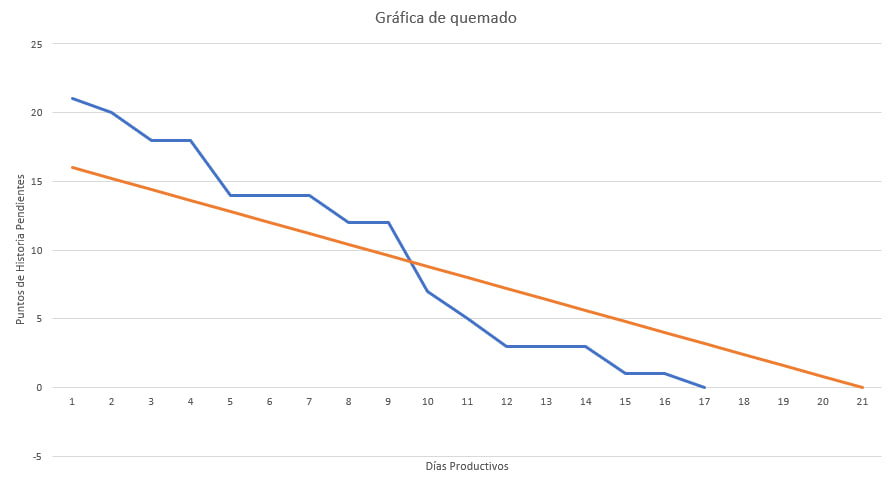
\includegraphics[height=10cm, width=15cm]{project/images/grafica.jpg}
  \caption{Gráfica de quemado del Sprint 1.}
  \label{fig:grafica_quemado}
\end{figure}

 % Especificación de requerimientos
\chapter{Arquitectura del sistema}

\section{Diseño general del sistema}

La arquitectura del sistema desarrollado para la plataforma comunitaria de Tejarcillos se basa en el patrón arquitectónico \textbf{Modelo-Vista-Controlador (MVC), lo que permite una separación clara de responsabilidades (Reenskaug, 1979).}, implementado sobre el stack tecnológico \textbf Se utilizó el stack MERN compuesto por MongoDB, Express.js, React y Node.js, tecnologías ampliamente utilizadas para el desarrollo web moderno (MongoDB, Inc., 2025; OpenJS Foundation, 2025a; OpenJS Foundation, 2025b; Meta Platforms, Inc., 2025b). Esta elección arquitectónica permite una separación clara de responsabilidades entre las diferentes capas del sistema, facilitando el mantenimiento, escalabilidad y comprensión del código.

El diseño de la comunicación cliente-servidor se implementó a través de una API RESTful, en línea con los principios planteados por Fielding (2000). La implementación sigue principios de desarrollo modular, donde cada componente tiene responsabilidades específicas y bien definidas.

\subsection*{Arquitectura Backend}
En el backend, la aplicación utiliza \textbf{Express.js con TypeScript} para aprovechar el tipado estático y mejorar la robustez del código. La estructura modular incluye:
\begin{itemize}
  \item \textbf{Controladores}: Gestionan la lógica de negocio y coordinan las operaciones entre modelos y rutas.
  \item \textbf{Modelos}: La persistencia de datos se gestiona mediante {Mongoose}, un ODM para MongoDB que facilita el manejo de esquemas (Automattic, 2025).
  \item \textbf{Rutas}: Definen los endpoints de la API REST y conectan las solicitudes HTTP con los controladores correspondientes.
  \item \textbf{Middlewares}: Proporcionan funcionalidades transversales como autenticación JWT, validación de roles y manejo de archivos.
  \item \textbf{Interfaces}: Definen contratos de datos utilizando TypeScript para garantizar consistencia.
\end{itemize}

\subsection*{Arquitectura Frontend}
El frontend está desarrollado en \textbf{React.js} utilizando componentes funcionales y \textbf{React Router} para la navegación. La estructura modular permite la reutilización de componentes y facilita el mantenimiento:
\begin{itemize}
  \item \textbf{Componentes reutilizables}: Elementos comunes de interfaz.
  \item \textbf{Páginas}: Vistas completas que integran múltiples componentes.
  \item \textbf{Servicios de API}: Centralizan las comunicaciones con el backend.
  \item \textbf{Context API}: Gestión del estado global de autenticación.
\end{itemize}

\subsection*{Comunicación y Seguridad}
La autenticación y autorización se implementó con JSON Web Tokens (JWT), siguiendo el estándar definido por la IETF (Jones, Bradley y Sakimura, 2015). El sistema implementa middleware de seguridad para validar roles de usuario y proteger rutas sensibles.

\subsection*{Mejoras en el Sprint 1}
Durante esta iteración se realizaron mejoras arquitectónicas significativas:
\begin{enumerate}
  \item \textbf{Sistema de categorías}: Se añadió una nueva entidad {Categoria} con su respectivo modelo, controlador y rutas.
  \item \textbf{Optimización del sistema de archivos}: Se mejoró la gestión de imágenes (servidor) y documentos (base de datos).
  \item \textbf{Calendario interactivo}: Integración con endpoints especializados para consultas por rangos de fechas.
  \item \textbf{Mejoras en la persistencia}: Nuevos campos en los modelos ({precio}, {horaEvento}) y referencias a categorías.
\end{enumerate}

\section{Diseño de la persistencia}

La persistencia se diseñó con un \textbf{modelo Entidad-Relación (E-R)} adaptado a MongoDB. Esta decisión permite aprovechar la flexibilidad de una base de datos orientada a documentos manteniendo claridad conceptual.

\subsection*{Modelo Conceptual Actualizado}
Cambios realizados en el Sprint 1:
\begin{itemize}
  \item \textbf{Usuario}: Se mantienen atributos originales ({nombre}, {apellidos}, {email}, {password}, {tipoUsuario}, {codigo}).
  \item {Publicación}: Se añadieron {precio} y {horaEvento}. Se reemplazó el campo {tag} por una referencia a {Categoria}.
  \item {Categoría (nueva)}: Incluye {identificador}, {nombre}, {tipo}. Relación uno a muchos con {Publicación}.
  \item {Comentario}: Sin cambios, mantiene relación con {Usuario} y {Publicación}.
  \item {Archivo y Carpeta}: Relaciones optimizadas y jerarquía mantenida.
\end{itemize}

\begin{figure}[H]
  \centering
    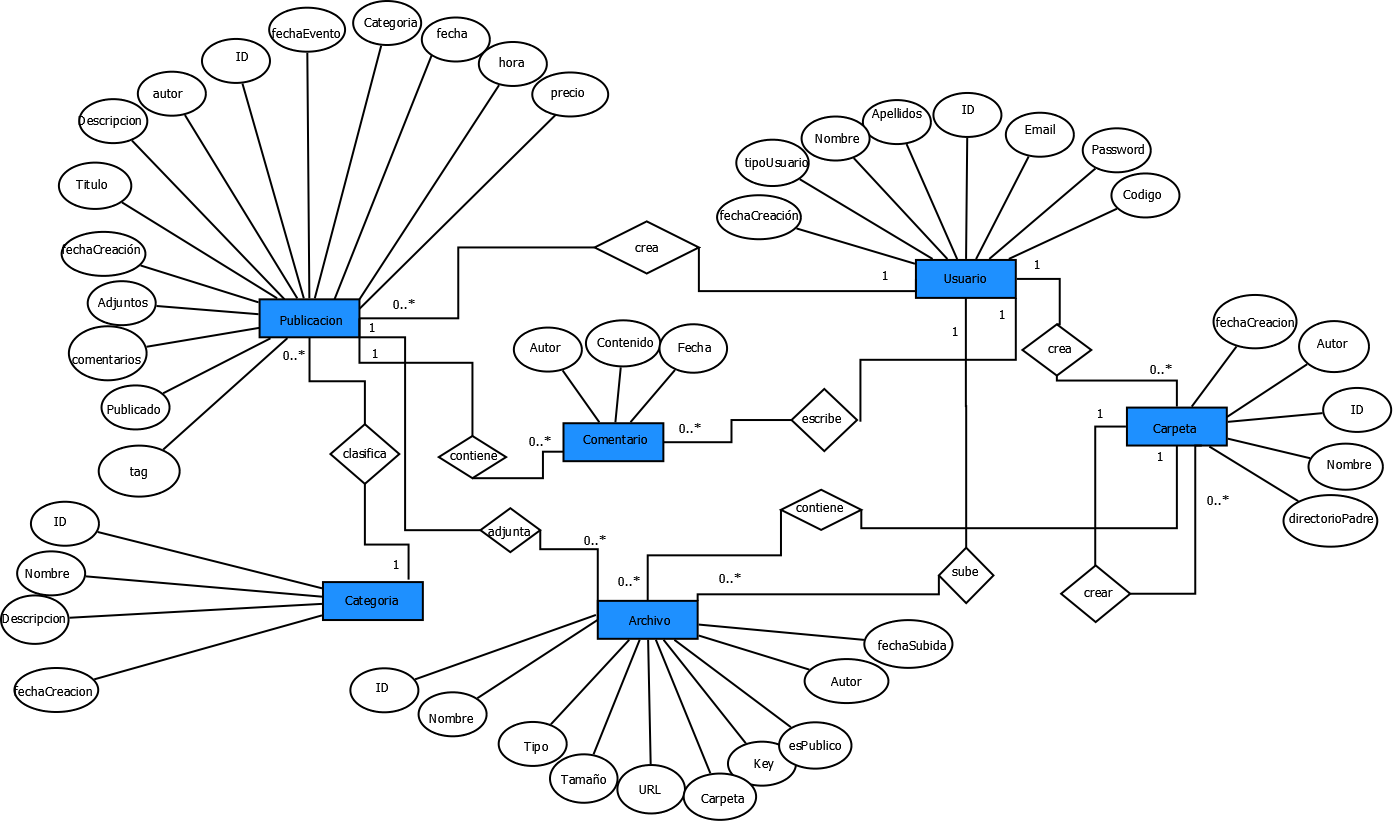
\includegraphics[width=15cm]{project/images/Diagrama1.png}
  \caption{\textbf{Modelo Entidad-Relación del sistema}}
  \label{ERModel}
\end{figure}

\subsection*{Justificación de los cambios}
\begin{enumerate}
  \item Migrar {tag} a entidad {Categoria} mejora integridad y eficiencia en consultas.
  \item Extensión de {Publicacion} permite cubrir emprendimientos y eventos sin nuevas entidades.
  \item Consultas más eficientes gracias a referencias y {populate} de Mongoose.
\end{enumerate}

\subsection*{Estrategia de Almacenamiento de Archivos}
\begin{itemize}
  \item \textbf{Imágenes}: En servidor local (\texttt{/srv/uploads}).
  \item \textbf{Documentos}: En MongoDB mediante GridFS.
\end{itemize}



\section{Diagrama de clases}

El diagrama de clases refleja la arquitectura orientada a objetos, actualizada tras las mejoras del Sprint 1. Incorpora la nueva clase {Categoria} y la extensión de {Publicacion}.

\subsection*{Clases principales}
\begin{itemize}
  \item \textbf{Usuario}: Atributos ({nombre}, {apellidos}, {email}, {password}, {tipoUsuario}, {codigo}). Relaciones: {Publicacion}, {Carpeta}, {Archivo}.
  \item \textbf{Categoria}: Atributos ({identificador}, {nombre}, {tipo}). Relación uno a muchos con {Publicacion}.
  \item \textbf{Publicacion}: Atributos ({titulo}, {contenido}, {fecha}, {adjuntos}, {comentarios}, {publicado}, {precio}, {horaEvento}). Asociación con {Categoria}.
  \item \textbf {Comentario}: Sin cambios, asociado a {Usuario} y {Publicacion}.
  \item \textbf {Archivo y Carpeta}: Mantienen estructura jerárquica y asociación con {Usuario}.
\end{itemize}

\subsection*{Mejoras en el diseño de clases}
\begin{enumerate}
  \item Separación de responsabilidades mediante la clase {Categoria}.
  \item Extensibilidad con nuevos campos en {Publicacion}.
  \item Integridad referencial en relación {Publicacion-Categoria}.
  \item Reutilización de categorías en múltiples publicaciones.
\end{enumerate}

\begin{figure}[H]
  \centering
    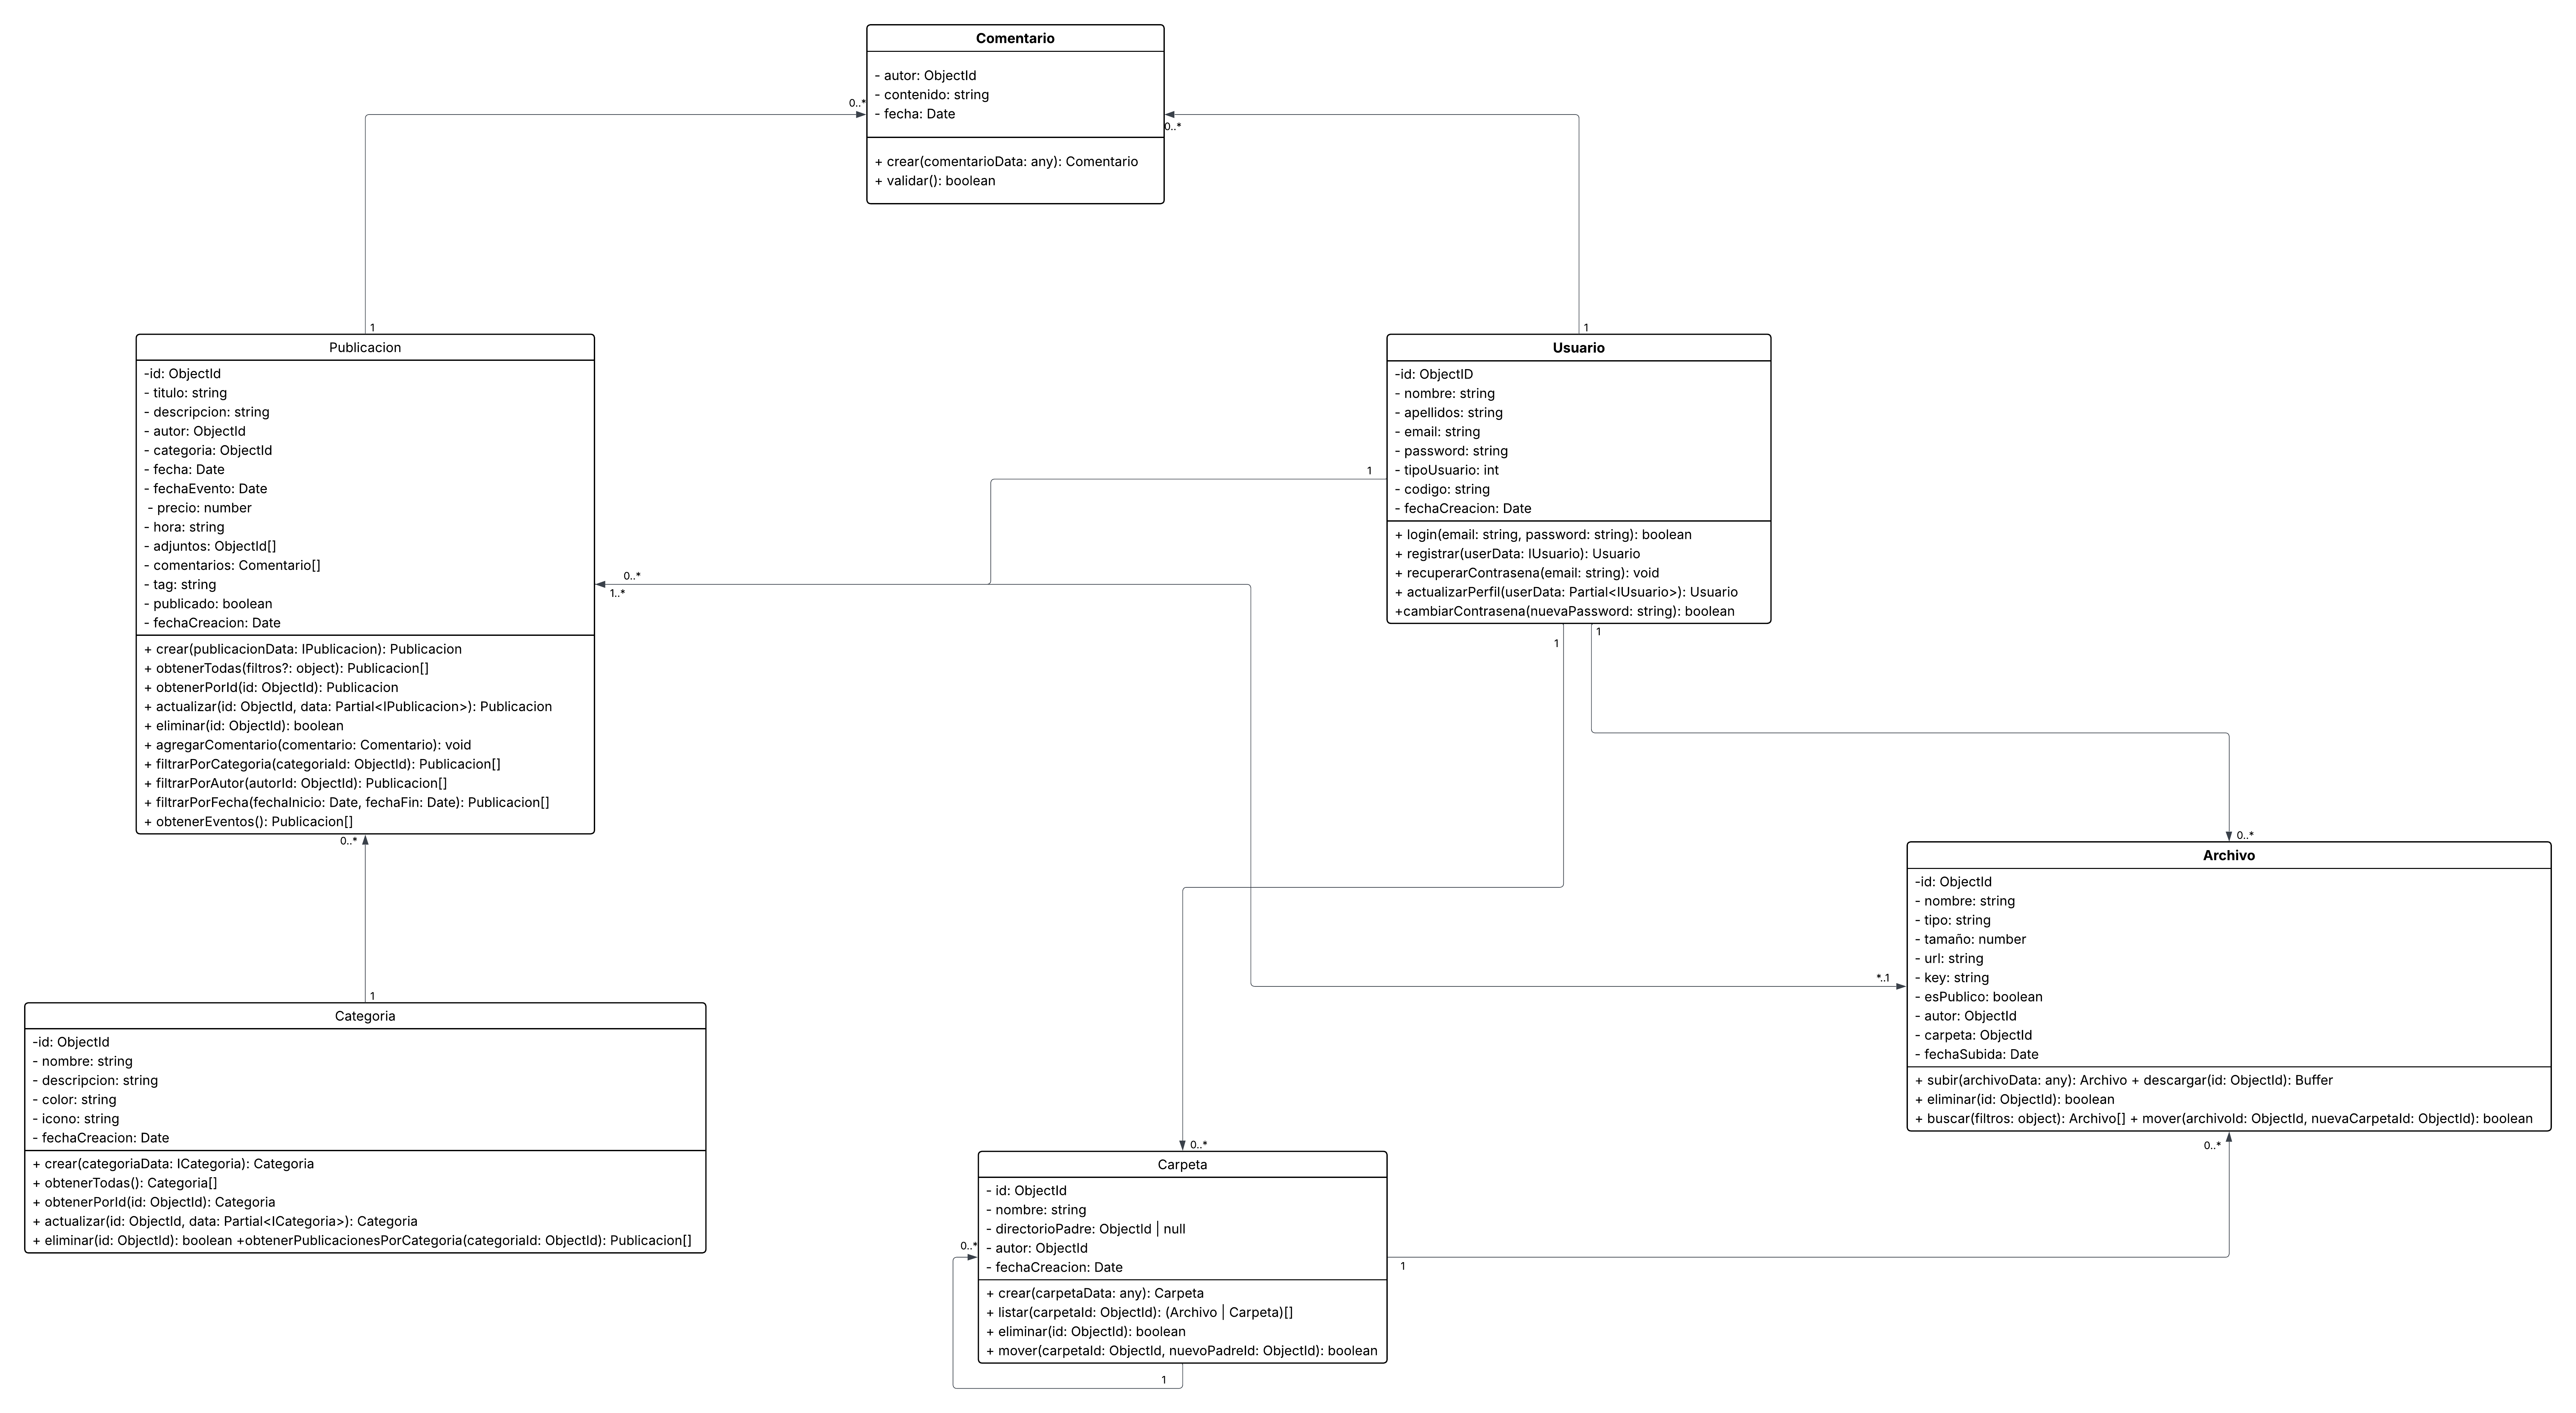
\includegraphics[width=15cm]{project/images/DC.png}
  \caption{\textbf{Diagrama de clases del sistema}}
  \label{DiagramaClases}
\end{figure}



 % Diseño del sistema
\chapter{Prototipos de interfaz}
En este capítulo se presentan los prototipos de interfaz desarrollados para el sistema \textbf{Komuness}, 
enfocándose en las funcionalidades implementadas y mejoradas durante el \textit{Sprint 1}. 
El diseño de la interfaz prioriza la usabilidad, accesibilidad y experiencia de usuario, considerando 
que el público objetivo son jóvenes de la comunidad de Tejarcillos, Alajuelita.

El enfoque de diseño se basa en principios de diseño centrado en el usuario, implementando interfaces intuitivas 
que no requieren conocimientos técnicos avanzados. Se ha prestado especial atención al diseño responsive, 
garantizando que la plataforma funcione correctamente en dispositivos móviles, tablets y computadoras de escritorio, 
ya que muchos usuarios de la comunidad acceden principalmente mediante smartphones.

\section{Prototipos de la funcionalidad de Sistema de Categorías}

El sistema de categorías implementado permite organizar el contenido por áreas temáticas específicas, 
facilitando la navegación y búsqueda de información relevante para los usuarios.

\subsection{Interfaz de Gestión de Categorías (Administrador)}

La Figura~\ref{fig:categorias-admin} muestra el panel de administración de categorías, 
donde los administradores pueden gestionar las clasificaciones temáticas del sistema.

\begin{figure}[H]
  \centering
  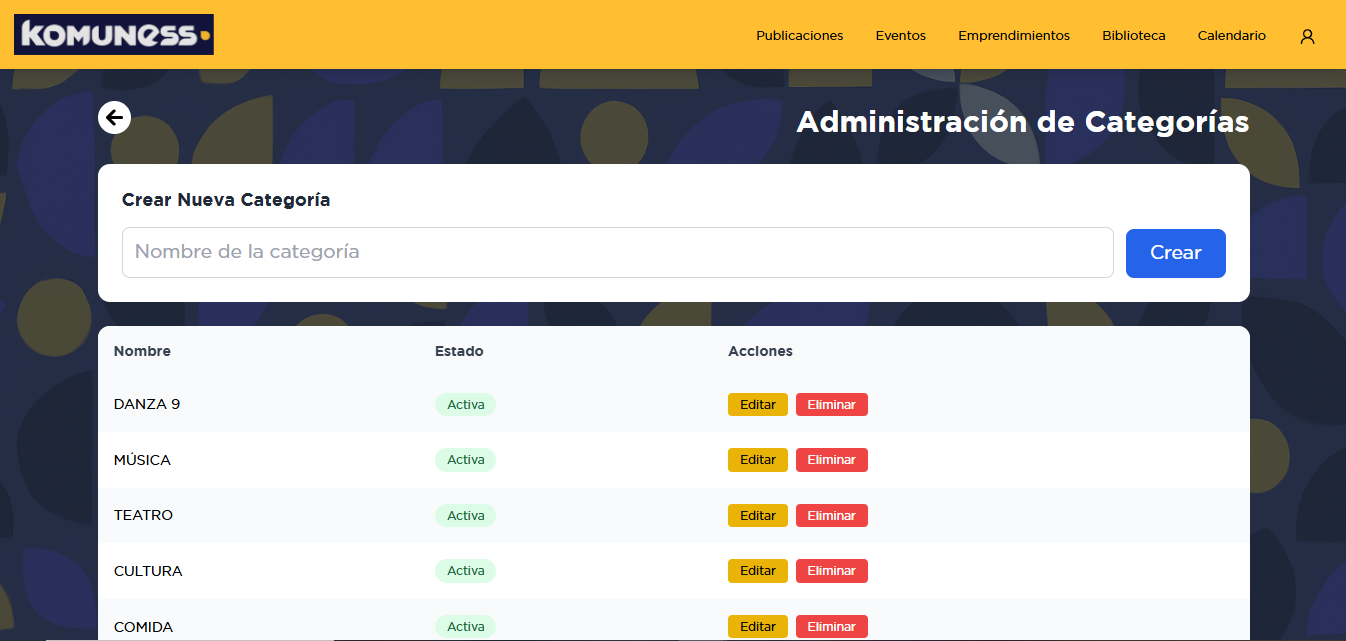
\includegraphics[width=0.9\textwidth]{project/images/imagen.PNG}
  \caption{Panel de administración de categorías - Vista principal con listado de categorías y opciones CRUD}
  \label{fig:categorias-admin}
\end{figure}

Características principales:
\begin{itemize}
  \item Vista tabular con opciones de crear, editar y eliminar.
  \item Formulario modal con campos: nombre, descripción y tipo.
  \item Validaciones en tiempo real para evitar duplicados.
  \item Confirmaciones de eliminación para prevenir pérdidas accidentales.
\end{itemize}

Características de usabilidad:
\begin{itemize}
  \item Botones con iconografía universal.
  \item Feedback visual inmediato (notificaciones de éxito/error).
  \item Búsqueda y filtrado en tiempo real.
  \item Diseño adaptativo para móviles y escritorio.
\end{itemize}

\subsection{Interfaz de Selección de Categorías (Usuario)}

La Figura~\ref{fig:categorias-selector} muestra cómo se integran las categorías en formularios de creación de publicaciones.

\begin{figure}[H]
  \centering
  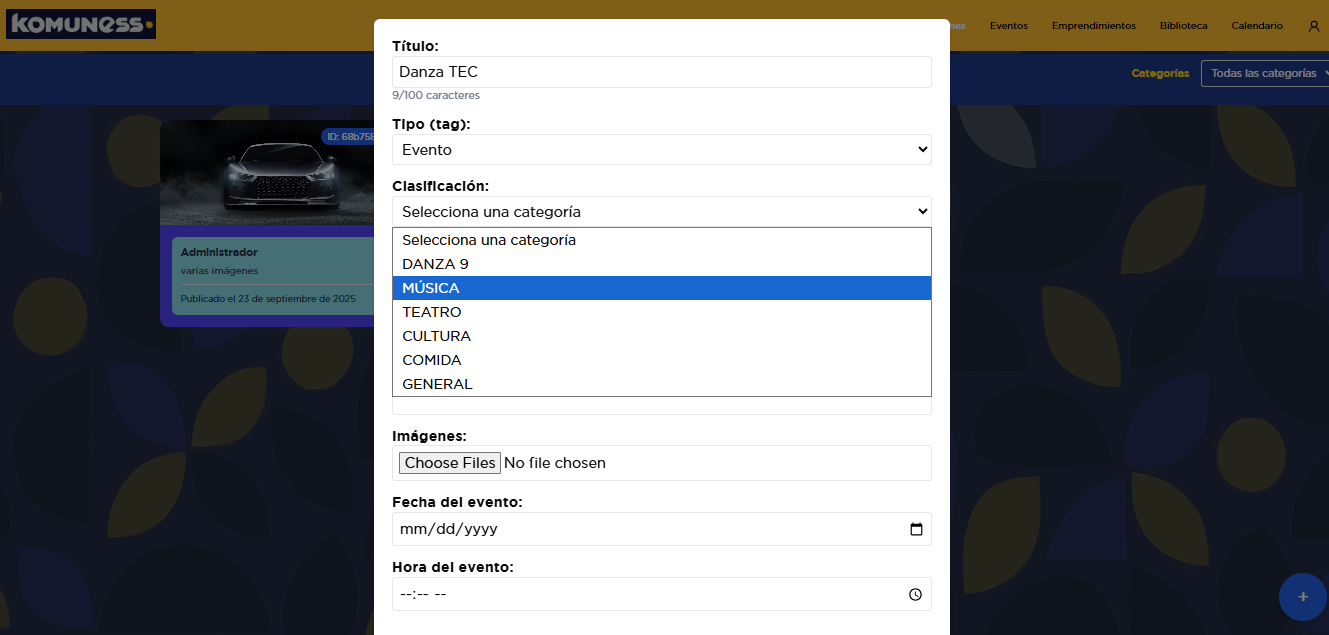
\includegraphics[width=0.8\textwidth]{project/images/imagen2.png}
  \caption{Selector de categorías integrado en formulario de creación de publicaciones}
  \label{fig:categorias-selector}
\end{figure}

\begin{itemize}
  \item Dropdown intuitivo integrado en formularios.
  \item Vista previa de la categoría seleccionada.
\end{itemize}

\begin{itemize}
  \item Badges visuales con categorías disponibles.
  \item Filtrado dinámico del contenido.
  \item Combinación de filtros (categoría + texto + autor).
  \item Indicador visual de filtros activos con opción de limpiar.
\end{itemize}

\begin{figure}[H]
  \centering
  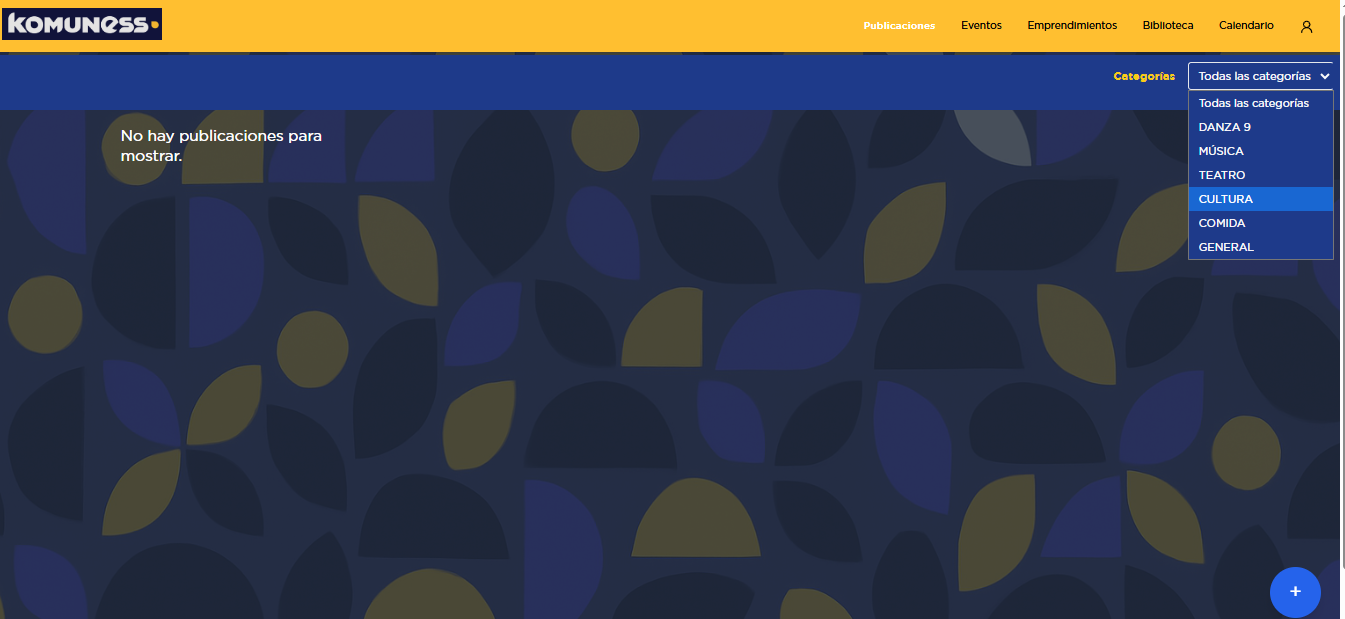
\includegraphics[width=0.9\textwidth]{project/images/imagen3.png}
  \caption{Sistema de filtros por categorías con badges visuales y filtrado dinámico}
  \label{fig:categorias-filtros}
\end{figure}

Principios de accesibilidad aplicados:
\begin{itemize}
  \item Contraste de colores (WCAG 2.1 AA).
  \item Texto alternativo en imágenes.
  \item Navegación completa por teclado.
  \item Tamaños de fuente escalables.
\end{itemize}

\section{Prototipos de la funcionalidad de Calendario Interactivo}

El calendario interactivo organiza eventos comunitarios, mejorando la participación en actividades.

\subsection{Vista Principal del Calendario}

La Figura~\ref{fig:calendario-vista} muestra la vista mensual del calendario.

\begin{figure}[H]
  \centering
  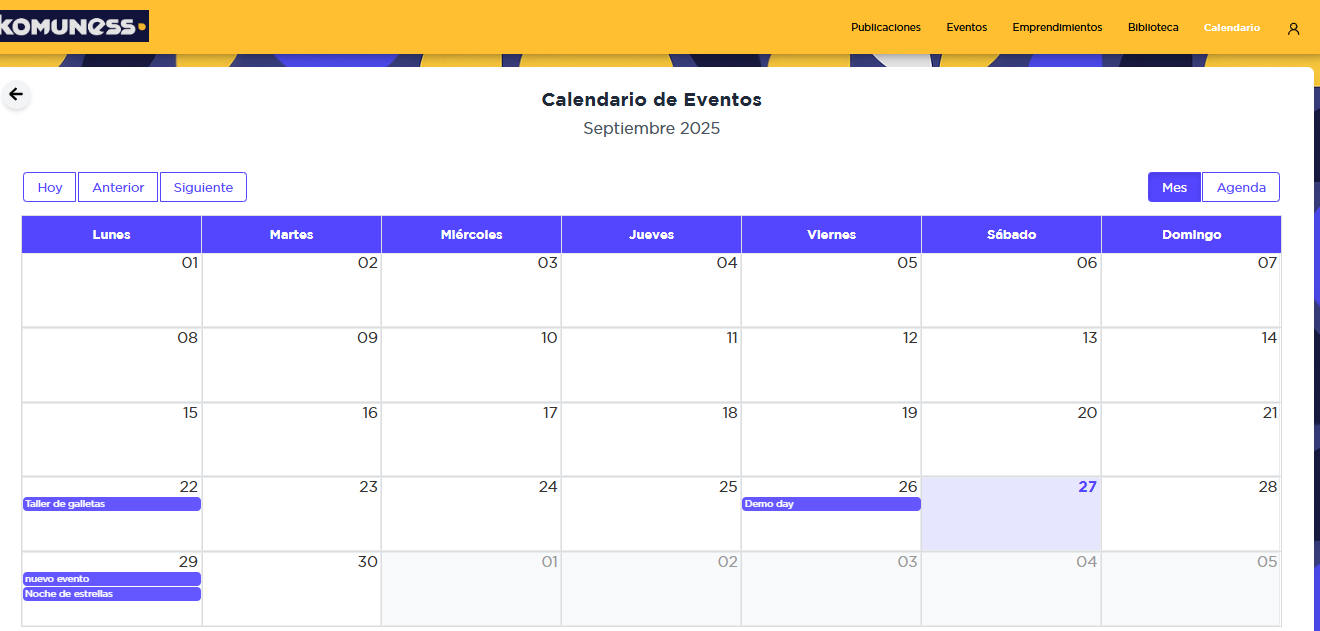
\includegraphics[width=0.9\textwidth]{project/images/imagen4.png}
  \caption{Vista principal del calendario interactivo con eventos marcados por fechas}
  \label{fig:calendario-vista}
\end{figure}

Características:
\begin{itemize}
  \item Layout en grid con eventos en fechas específicas.
  \item Navegación por meses (anterior/siguiente).
  \item Indicadores visuales por tipo de evento.
  \item Hover con información básica del evento.
\end{itemize}

\subsection{Vista de agenda}

La Figura~\ref{fig:calendario-detalle} muestra el panel lateral  eventos proximo.

\begin{figure}[H]
  \centering
  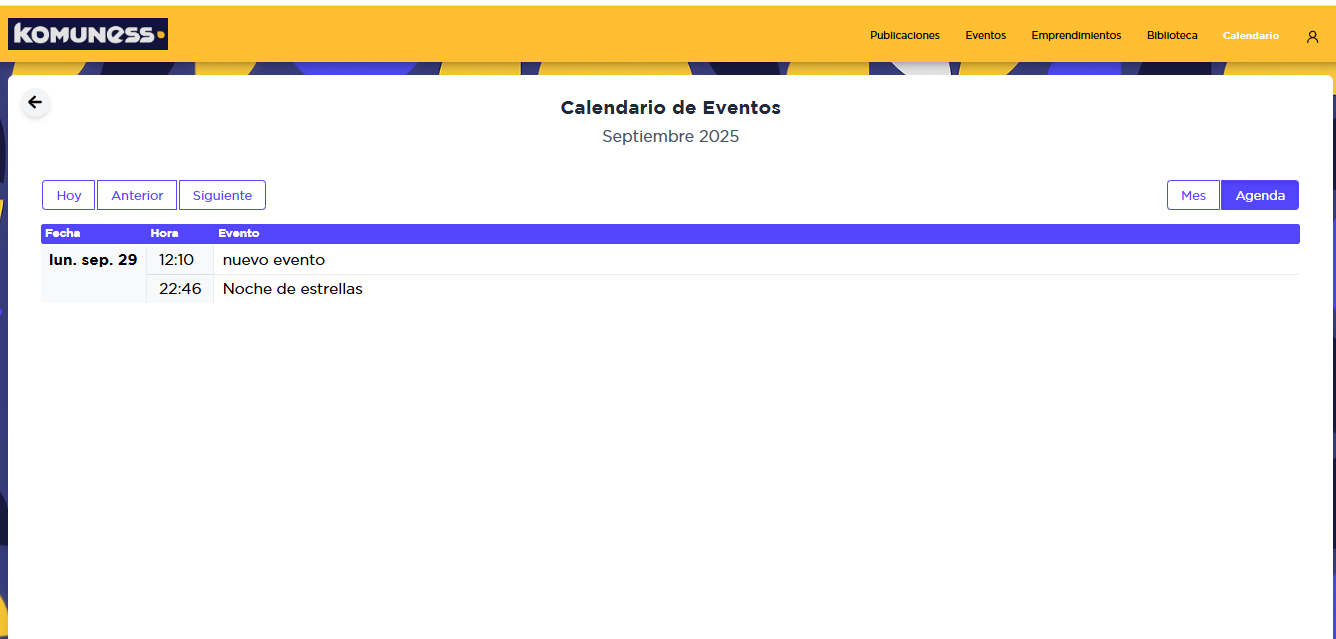
\includegraphics[width=0.8\textwidth]{project/images/imagen5.PNG}
  \caption{Panel de agenda de eventos con campos especificos}
  \label{fig:calendario-detalle}
\end{figure}

\begin{itemize}
  \item Información: fecha, hora, evento.

\end{itemize}

\subsection{Creación de Eventos}

La Figura~\ref{fig:calendario-crear} muestra el formulario de creación de eventos.

\begin{figure}[H]
  \centering
  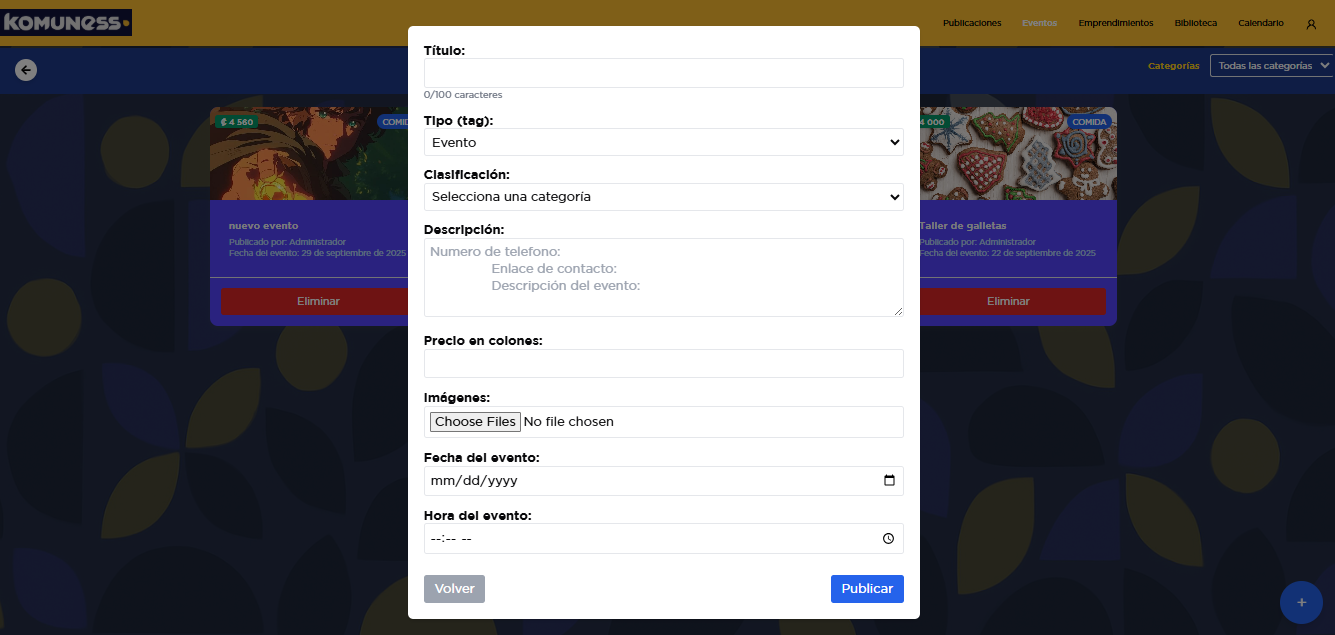
\includegraphics[width=0.85\textwidth]{project/images/imagen6.PNG}
  \caption{Formulario especializado para creación de eventos}
  \label{fig:calendario-crear}
\end{figure}

\begin{itemize}
  \item Campos: Titulo, Tag, Clasificación,Descripcion, Imagenes, Fecha del evento, Hora del evento.
  \item Validaciones: no permitir eventos sin información completa.
  \item Preview en tiempo real.
\end{itemize}

\subsection{Biblioteca Digital Optimizada}

Figura~\ref{fig:biblioteca} muestra la nueva vista con sistema de carpetas y filtros.

\begin{figure}[H]
  \centering
  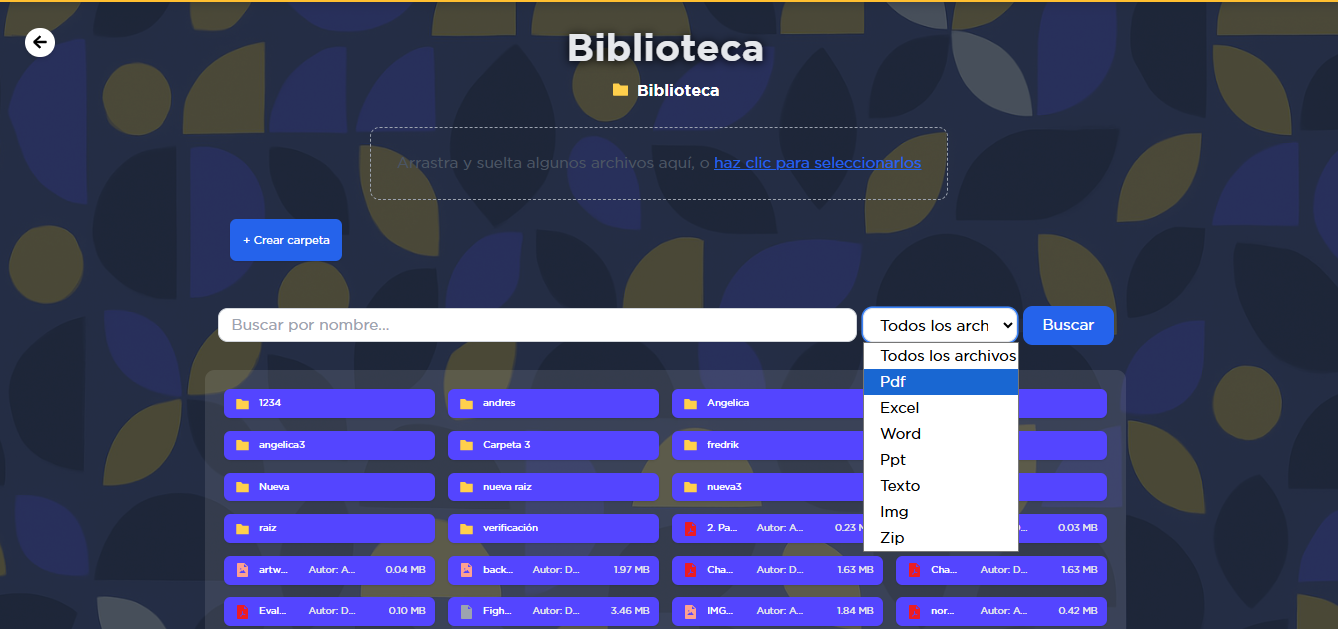
\includegraphics[width=0.9\textwidth]{project/images/imagen7.png}
  \caption{Vista de biblioteca digital optimizada con carpetas y filtros de búsqueda}
  \label{fig:biblioteca}
\end{figure}

\subsection{Diseño Responsive}

La Figura~\ref{fig:responsive} muestra la adaptación a distintos dispositivos.

\begin{figure}[H]
  \centering
  % Opción 1: ancho fijo en centímetros
  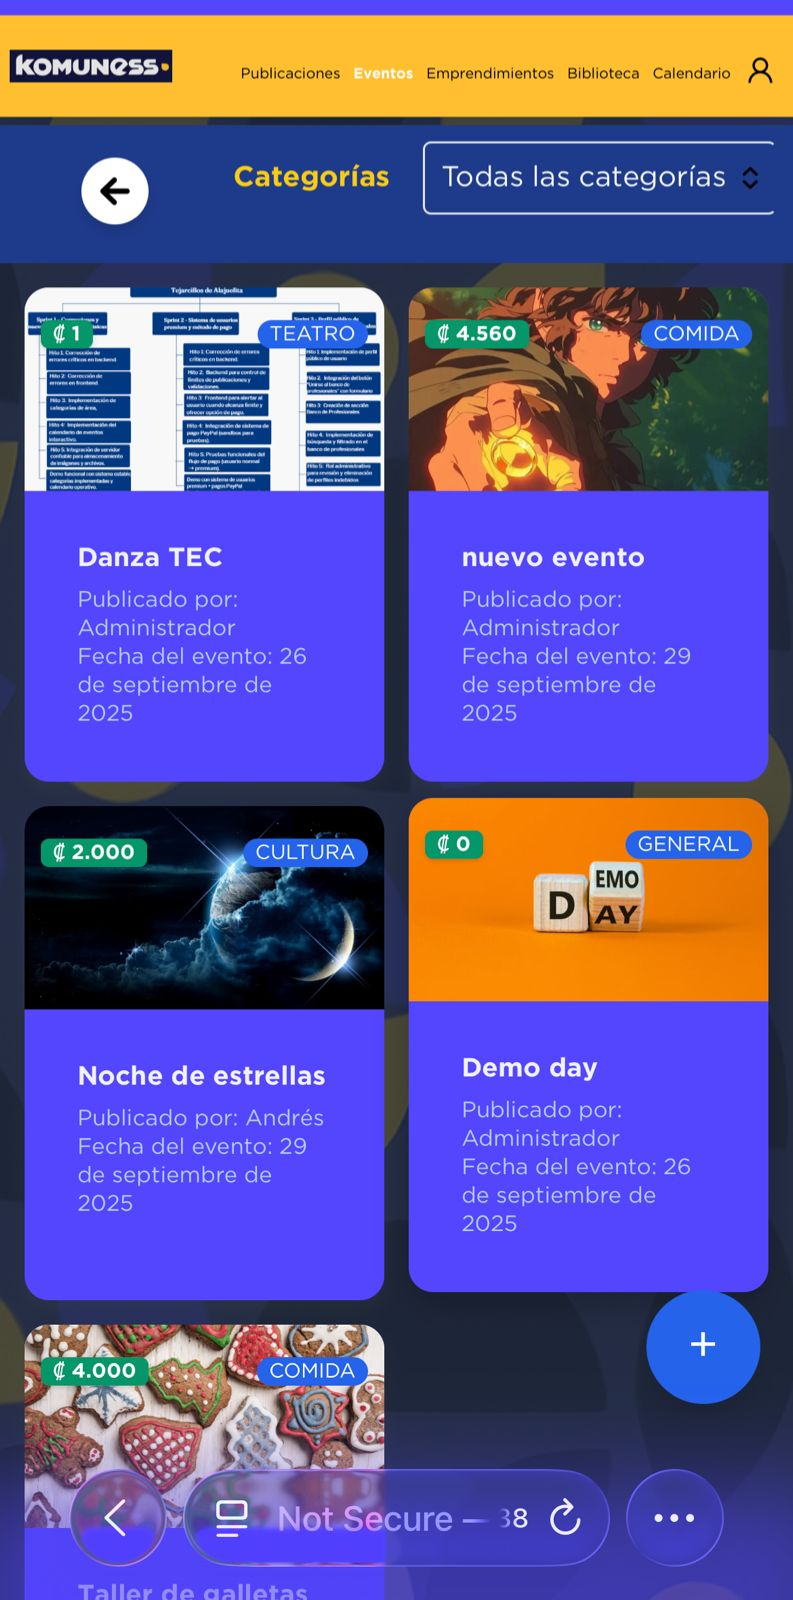
\includegraphics[width=4cm,keepaspectratio]{project/images/imagen8.jpg}
  
  % Opción 2: usar scale (reduce al 20% del tamaño original)
  %\includegraphics[scale=0.2]{project/images/responsive}

  % Opción 3: limitar ancho y alto para que nunca sea inmensa
  %\includegraphics[width=6cm,height=10cm,keepaspectratio]{project/images/responsive}

  \caption{Vista responsive en dispositivos móviles}
  \label{fig:responsive}
\end{figure}


\subsection{Características de Diseño y Usabilidad}

\begin{itemize}
  \item Transiciones suaves entre vistas.
  \item Estados de carga y vacíos informativos.
  \item Iconografía clara y culturalmente relevante.
  \item Touch targets grandes para móviles.
  \item Mensajes de error claros y confirmaciones visuales.
\end{itemize}
 % Prototipos de interfaz de usuario
\chapter{Control de calidad}

El proceso de control de calidad implementado en el proyecto \textbf{Komuness} durante el Sprint 1 se enfocó en garantizar la estabilidad, funcionalidad y usabilidad del sistema mediante una estrategia integral que combina pruebas manuales, automatizadas y validaciones de usuario final. 

El equipo adoptó un enfoque de \textit{testing} continuo, donde cada funcionalidad implementada fue sometida a múltiples niveles de verificación antes de su integración al sistema principal.

La estrategia de control de calidad se estructuró en tres pilares fundamentales:
\begin{itemize}
    \item \textbf{Pruebas funcionales:} verificación de que cada requerimiento cumple con las especificaciones.
    \item \textbf{Pruebas de integración:} validación de la comunicación entre componentes.
    \item \textbf{Pruebas de usabilidad:} confirmación de que las interfaces son intuitivas y accesibles para el público objetivo.
\end{itemize}

\section{Equipo participante}
Los miembros involucrados en el proceso de control de calidad fueron:
\begin{itemize}
    \item \textbf{Fredrik Aburto Jiménez} 
    \item \textbf{Angélica Díaz Barrios} 
    \item \textbf{Andrés Salas Araya} 
\end{itemize}

\section{Herramientas utilizadas}
Se emplearon diversas herramientas y entornos para garantizar la calidad:
\begin{itemize}
    \item \textbf{Postman:} pruebas automatizadas de endpoints API y validación de respuestas HTTP (fielding2000).
   \item \textbf{Jest + Supertest:} framework de pruebas unitarias y de integración para backend en Node.js (openjsnode2025).
  \item \textbf{Navegadores múltiples:} validación cross-browser (Chrome, Firefox, Safari, Edge) (microsoft2025).
  \item \textbf{Dispositivos físicos:} validación en smartphones y tablets reales para pruebas responsive.

\end{itemize}

\section{Guiones de pruebas}

Se desarrollaron \textbf{8 guiones de pruebas específicos} para validar las funcionalidades críticas implementadas durante el Sprint 1.  
Los criterios empleados fueron:
\begin{itemize}
    \item Cobertura funcional completa (cada requerimiento con al menos una prueba).
    \item Escenarios de borde (validación de casos límite y manejo de errores).
    \item Flujos de usuario reales (simulación de comportamientos típicos).
    \item Compatibilidad cross-platform (funcionamiento en distintos dispositivos y navegadores).
\end{itemize}

\subsection{Guión 1: Sistema de Categorías (RF001, RF004, RF007)}

\begin{longtable}{ | p{2cm} | p{4cm} | p{4cm} | p{4cm} | c |}
\hline
\textbf{Historias} & \textbf{Descripción} & \textbf{Resultado Esperado} & \textbf{Resultado Obtenido} & \textbf{Condición}\\
\hline
RF001 y RF004 & Creación de categoría nueva desde panel admin con nombre ``MUSICA'' & Categoría creada exitosamente, aparece en listado de admin y disponible en selectores de usuario & Categoría creada correctamente, validación de duplicados funcionando, integración completa con frontend & \color{ForestGreen}PASÓ \\
\hline
RF004 y RF007 & Eliminación de categoría con publicaciones asociadas & Sistema debe mostrar advertencia y prevenir eliminación, o reasignar publicaciones & Advertencia mostrada correctamente, eliminación bloqueada cuando hay dependencias & \color{ForestGreen}PASÓ \\
\hline
RF007 & Filtrado de publicaciones por categoría ``Cultura'' & Solo publicaciones de esa categoría se muestran con indicador visual de filtro activo & Filtrado funcionando correctamente, badges implementados, combinación con otros filtros operativa & \color{ForestGreen}PASÓ \\
\hline
\caption{Guión de pruebas 1: Sistema de categorías}
\label{TestScript1}
\end{longtable}

\subsection{Guión 2: Calendario Interactivo (RF005, RF009)}

\begin{longtable}{ | p{2cm} | p{4cm} | p{4cm} | p{4cm} | c |}
\hline
\textbf{Historias} & \textbf{Descripción} & \textbf{Resultado Esperado} & \textbf{Resultado Obtenido} & \textbf{Condición}\\
\hline
RF005 & Navegación entre meses y visualización de eventos & Transición fluida y eventos en fechas correctas con indicadores visuales & Navegación funcionando, eventos renderizados correctamente & \color{ForestGreen}PASÓ \\
\hline
RF009 & Creación de evento con precio ₡5000 y hora 2:00 PM & Evento guardado con datos completos, mostrado en calendario y detalles & Persistencia en BD correcta, visualización completa en calendario y detalles & \color{ForestGreen}PASÓ \\
\hline
RF005 y RF009 & Visualización de detalles de evento & Modal/panel muestra título, descripción, fecha, hora, precio, categoría & Detalles completos, formato correcto de hora y precio & \color{ForestGreen}PASÓ \\
\hline
\caption{Guión de pruebas 2: Calendario interactivo}
\label{TestScript2}
\end{longtable}

\subsection{Guión 3: Sistema de Archivos (RF003, RF008)}

\begin{longtable}{ | p{2cm} | p{4cm} | p{4cm} | p{4cm} | c |}
\hline
\textbf{Historias} & \textbf{Descripción} & \textbf{Resultado Esperado} & \textbf{Resultado Obtenido} & \textbf{Condición}\\
\hline
RF003 & Subida de imagen JPG de 2MB a publicación & Imagen subida a Digital Ocean, URL generada y asociada a publicación & Subida exitosa y visualización correcta & \color{ForestGreen}PASÓ \\
\hline
RF008 & Subida de documento PDF de 5MB a biblioteca & Archivo almacenado en servidor, metadata guardada en BD & Almacenamiento local correcto, metadata completa y descarga operativa & \color{ForestGreen}PASÓ \\
\hline
RF008 & Creación de carpeta ``Documentos 2025'' y subida en ella & Carpeta creada, archivo en jerarquía & Jerarquía funcionando, navegación operativa & \color{ForestGreen}PASÓ \\
\hline
\caption{Guión de pruebas 3: Sistema de archivos}
\label{TestScript3}
\end{longtable}

\subsection{Guión 4: Optimizaciones Frontend (RF002, RF010)}

\begin{longtable}{ | p{2cm} | p{4cm} | p{4cm} | p{4cm} | c |}
\hline
\textbf{Historias} & \textbf{Descripción} & \textbf{Resultado Esperado} & \textbf{Resultado Obtenido} & \textbf{Condición}\\
\hline
RF002 & Navegación entre vistas principales & Todas las rutas funcionan, botones ``Volver'' operativos & Navegación fluida y sin errores de rutas & \color{ForestGreen}PASÓ \\
\hline
RF010 & Visualización en móvil (320px) & Interfaz adaptada, sin superposición, texto legible & Responsive design funcionando correctamente & \color{ForestGreen}PASÓ \\
\hline
RF010 & Manejo de errores en subida de archivos & Mensajes de error claros y orientativos & Feedback visual correcto, guías de solución mostradas & \color{ForestGreen}PASÓ \\
\hline
\caption{Guión de pruebas 4: Optimizaciones frontend}
\label{TestScript4}
\end{longtable}

\subsection{Guión 5: Autenticación y Seguridad (RNF001)}

\begin{longtable}{ | p{2cm} | p{4cm} | p{4cm} | p{4cm} | c |}
\hline
\textbf{Historias} & \textbf{Descripción} & \textbf{Resultado Esperado} & \textbf{Resultado Obtenido} & \textbf{Condición}\\
\hline
RNF001 & Login con credenciales válidas & Usuario autenticado, JWT generado, redirección a dashboard & Autenticación exitosa, token válido, sesión persistente & \color{ForestGreen}PASÓ \\
\hline
RNF001 & Acceso a ruta protegida sin login & Redirección a login con mensaje informativo & Middleware funcionando, redirección correcta & \color{ForestGreen}PASÓ \\
\hline
RNF001 & Logout e invalidación de sesión & Sesión cerrada, token invalidado, redirección a inicio & Logout funcionando, cookie removida & \color{ForestGreen}PASÓ \\
\hline
\caption{Guión de pruebas 5: Autenticación y seguridad}
\label{TestScript5}
\end{longtable}
 % Pruebas
\chapter{Capturas de pantalla}

Este capítulo presenta capturas de pantalla del sistema \textbf{Komuness} implementado, documentando visualmente el progreso alcanzado durante el Sprint 1. 
Las imágenes proporcionan evidencia tangible de las funcionalidades desarrolladas y sirven como registro del estado actual de la plataforma para futuras iteraciones.

Las capturas están organizadas por funcionalidad principal, mostrando tanto la perspectiva del usuario final como las interfaces administrativas. 
Se incluyen vistas en diferentes dispositivos para demostrar la implementación responsive y la adaptabilidad del sistema a diversos contextos de uso.

\section{Capturas del Sistema de Categorías}

Esta sección documenta la implementación completa del sistema de categorías, desde la gestión administrativa hasta la experiencia del usuario final en la clasificación y filtrado de contenido.

\subsection*{Gestión Administrativa de Categorías}

\begin{figure}[H]
  \centering
  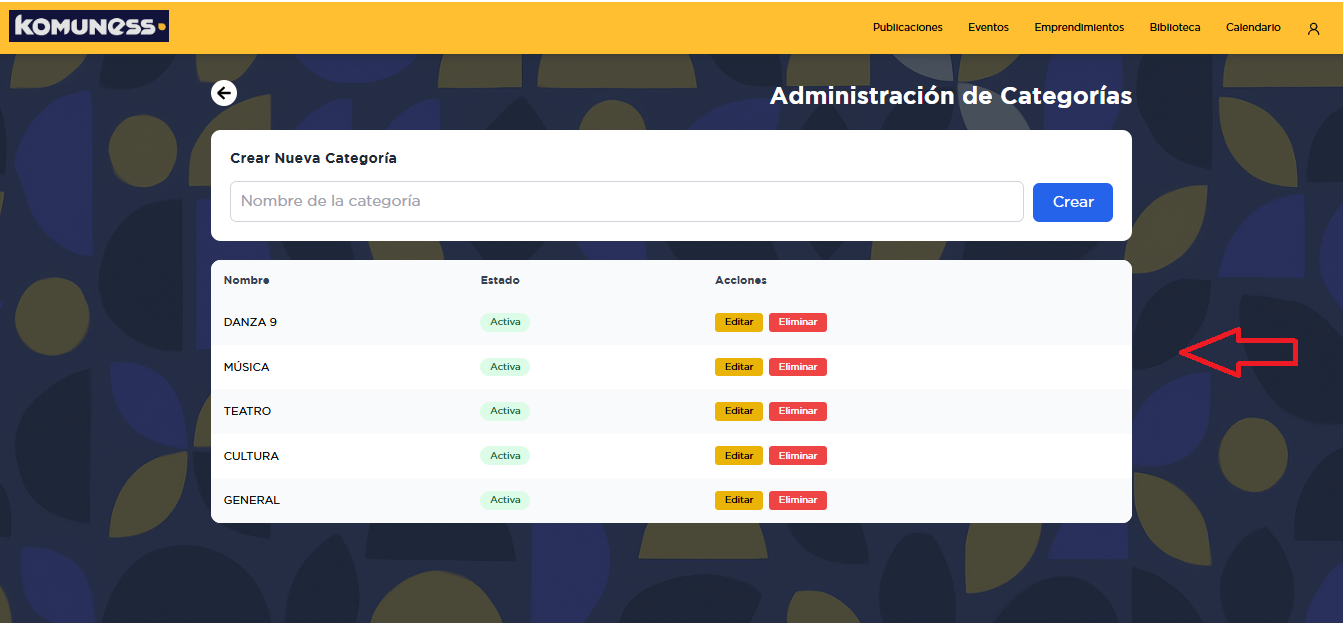
\includegraphics[width=\textwidth]{project/images/6.1.png}
  \caption{Vista principal del panel de administración de categorías mostrando el listado completo con opciones CRUD}
  \label{fig:cat-admin}
\end{figure}

\begin{figure}[H]
  \centering
  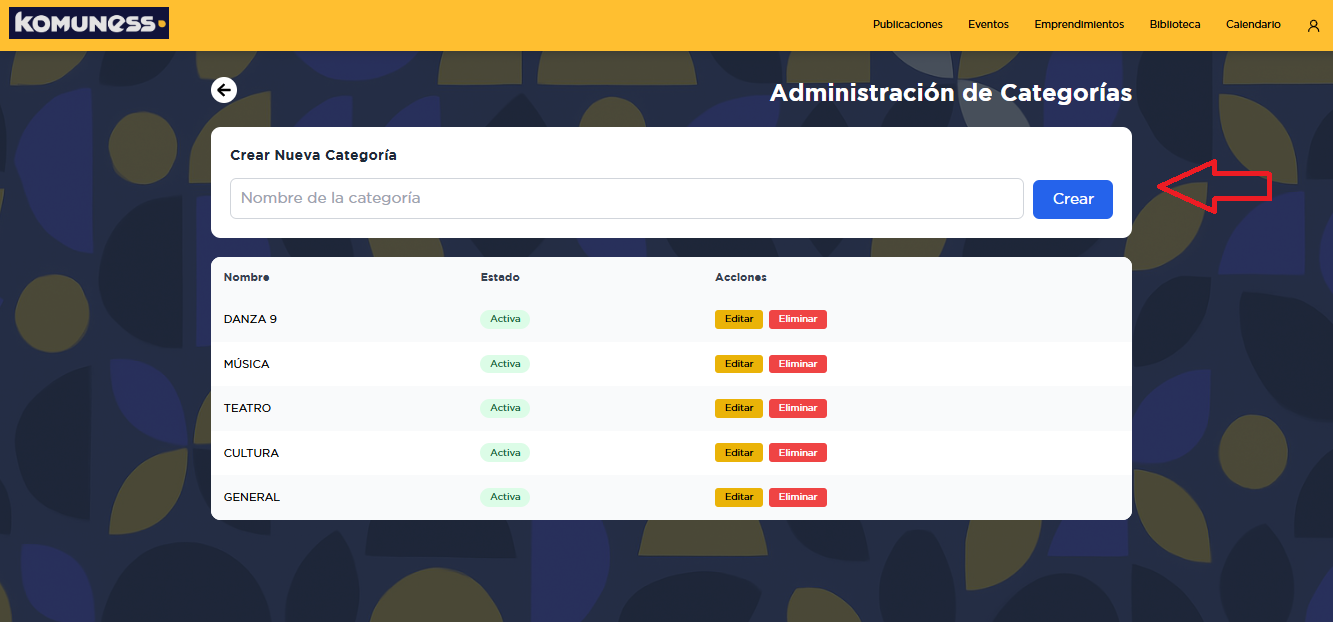
\includegraphics[width=\textwidth]{project/images/6.2.png}
  \caption{Modal de creación de nueva categoría con formulario de validación}
  \label{fig:cat-modal}
\end{figure}

\begin{figure}[H]
  \centering
  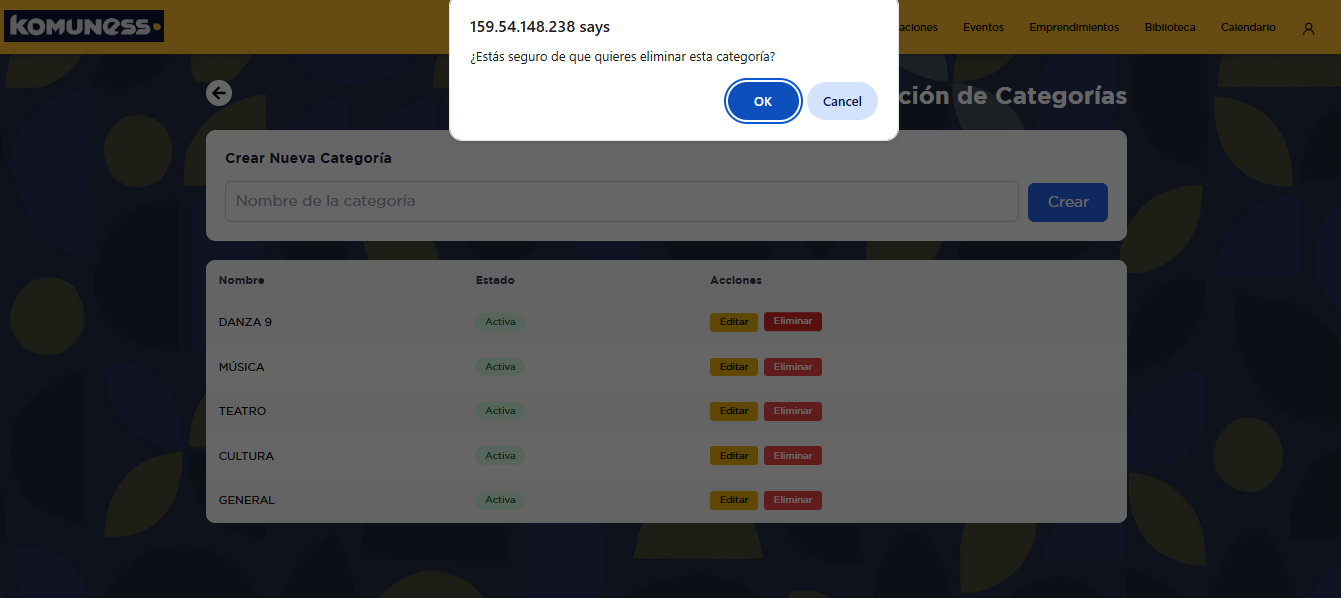
\includegraphics[width=\textwidth]{project/images/6.3.png}
  \caption{Confirmación de eliminación de categoría con advertencia de dependencias}
  \label{fig:cat-delete}
\end{figure}

\subsection*{Experiencia del Usuario con Categorías}

\begin{figure}[H]
  \centering
  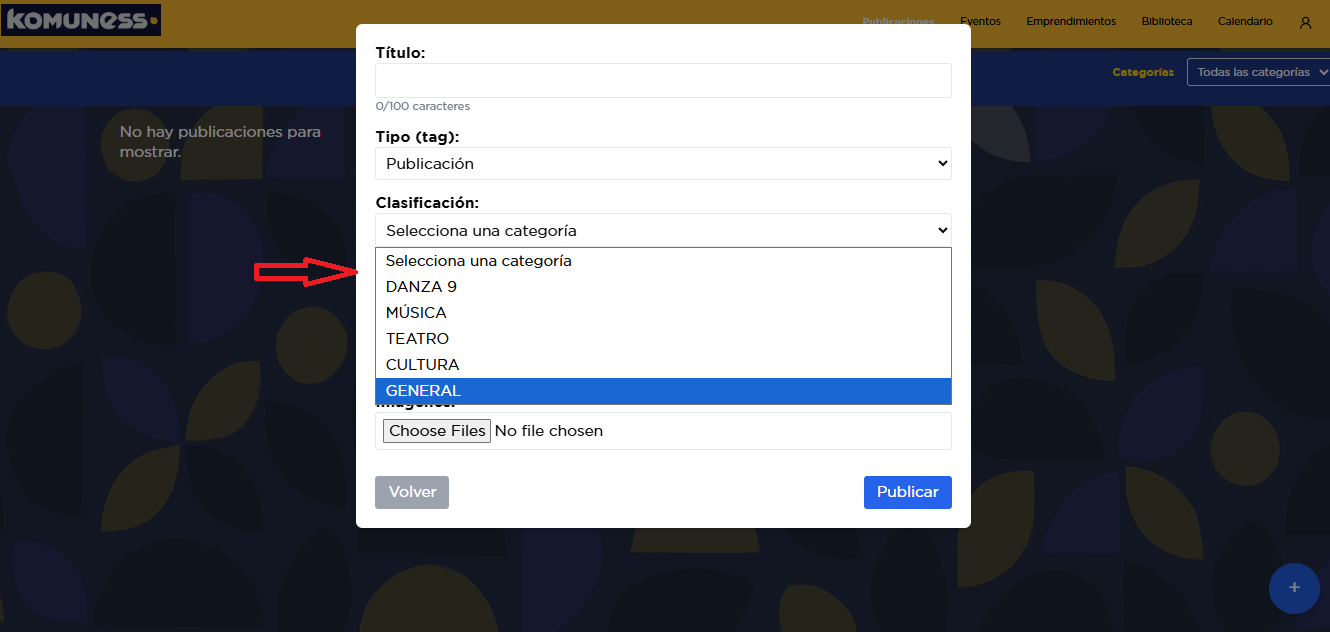
\includegraphics[width=\textwidth]{project/images/6.4.png}
  \caption{Selector de categorías integrado en formulario de creación de publicaciones}
  \label{fig:cat-selector}
\end{figure}


\begin{figure}[H]
  \centering
  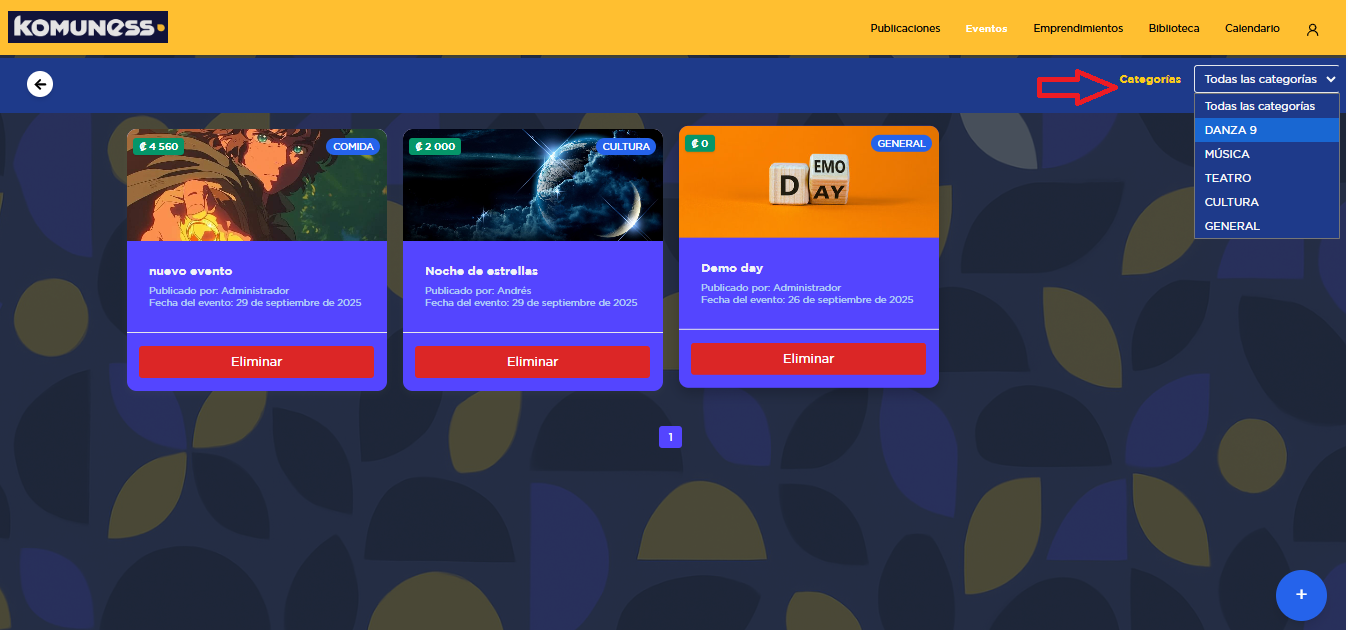
\includegraphics[width=\textwidth]{project/images/6.5.png}
  \caption{Vista de publicaciones filtradas por categoría específica}
  \label{fig:cat-filtradas}
\end{figure}

\section{Capturas del Calendario Interactivo}

\subsection*{Vista Principal del Calendario}

\begin{figure}[H]
  \centering
  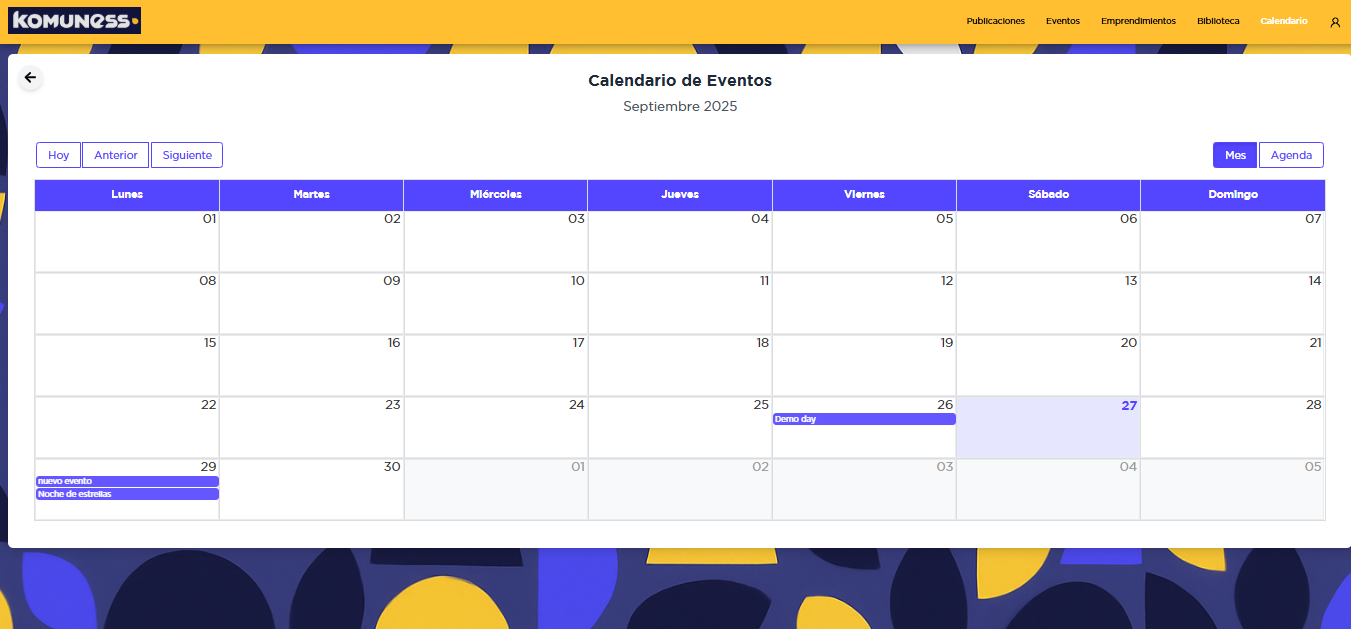
\includegraphics[width=\textwidth]{project/images/6.9.png}
  \caption{Vista mensual del calendario con eventos marcados por fechas}
  \label{fig:cal-mensual}
\end{figure}


\subsection*{Detalles y Gestión de Eventos}

\begin{figure}[H]
  \centering
  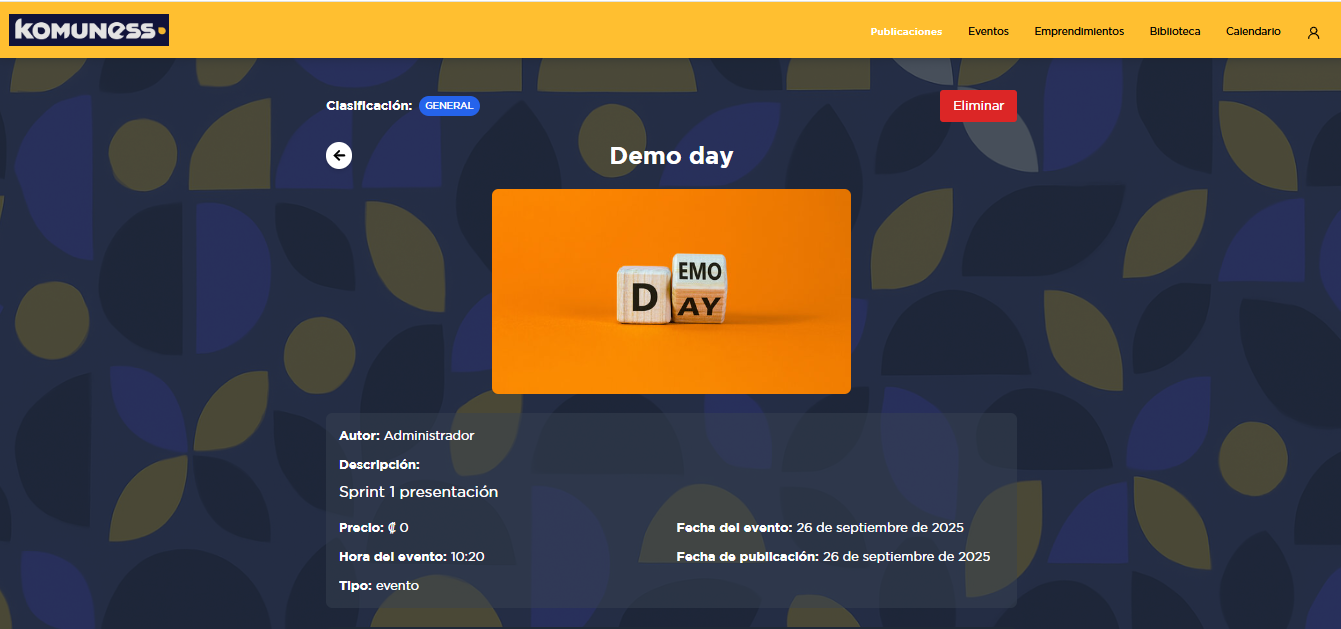
\includegraphics[width=\textwidth]{project/images/6.7.png}
  \caption{Panel de detalles de evento mostrando información completa}
  \label{fig:cal-detalles}
\end{figure}

\begin{figure}[H]
  \centering
  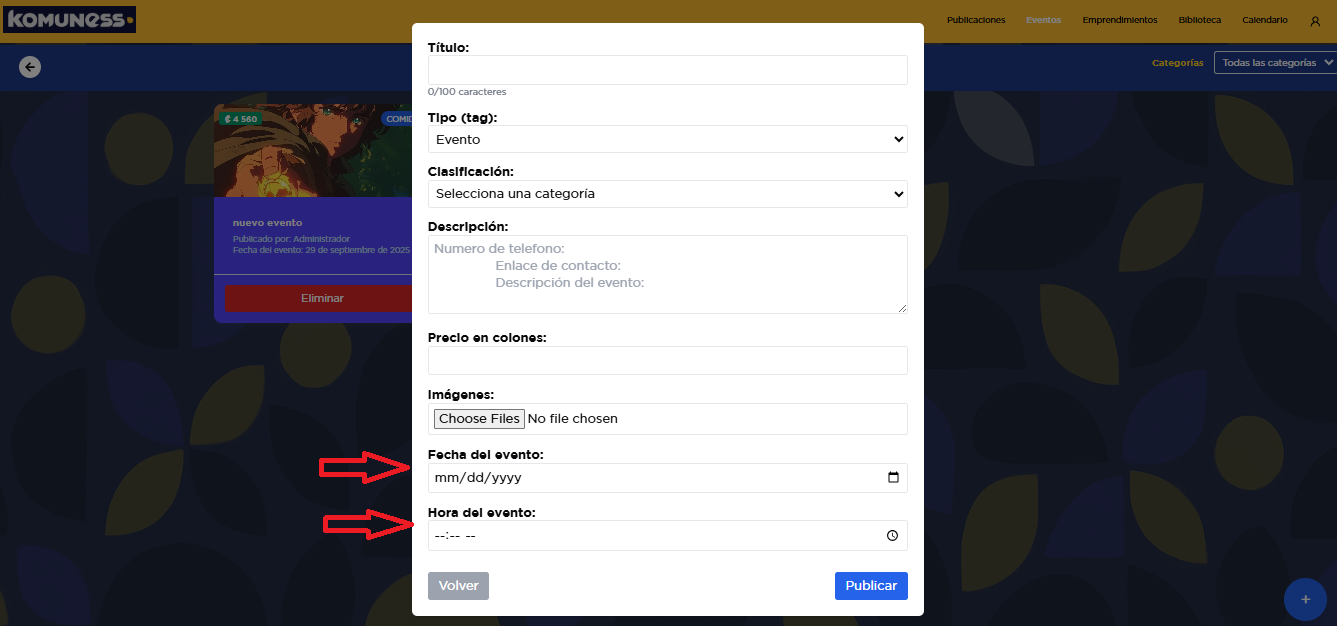
\includegraphics[width=\textwidth]{project/images/6.8.png}
  \caption{Formulario especializado para creación de eventos con campos precio y hora}
  \label{fig:cal-form}
\end{figure}

\begin{figure}[H]
  \centering
  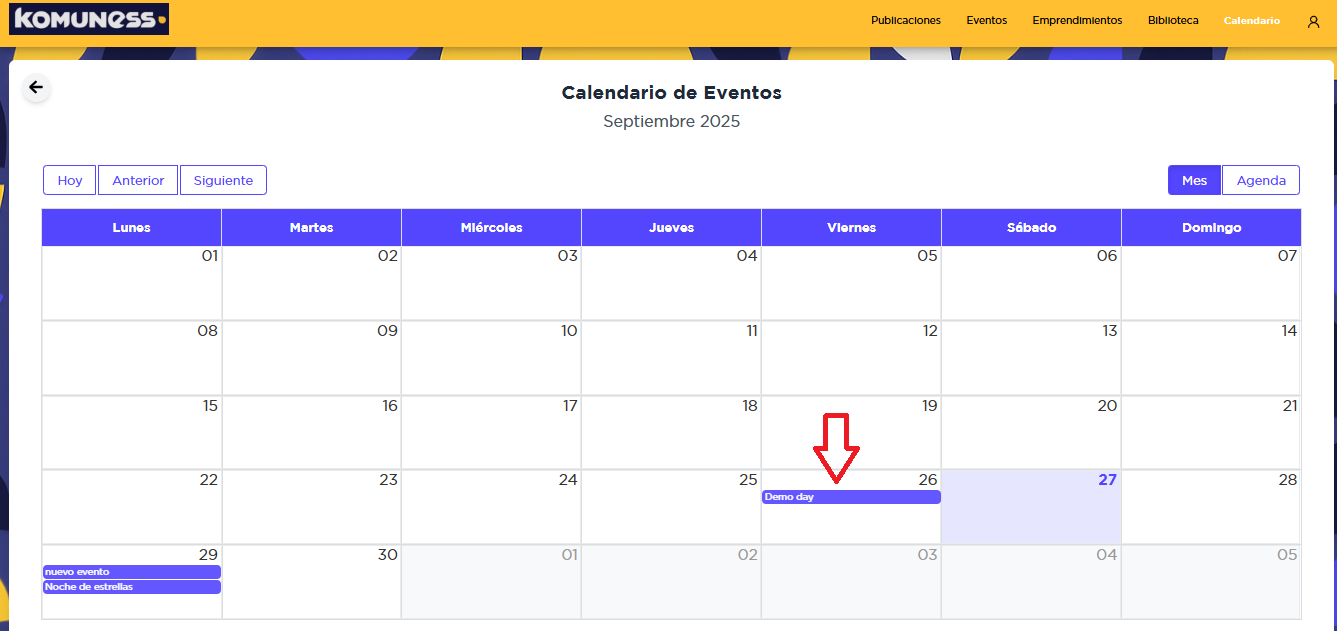
\includegraphics[width=\textwidth]{project/images/6.6}
  \caption{Vista de evento en calendario con dia visible}
  \label{fig:cal-evento}
\end{figure}


\section{Capturas de Mejoras en Biblioteca Digital}

\begin{figure}[H]
  \centering
  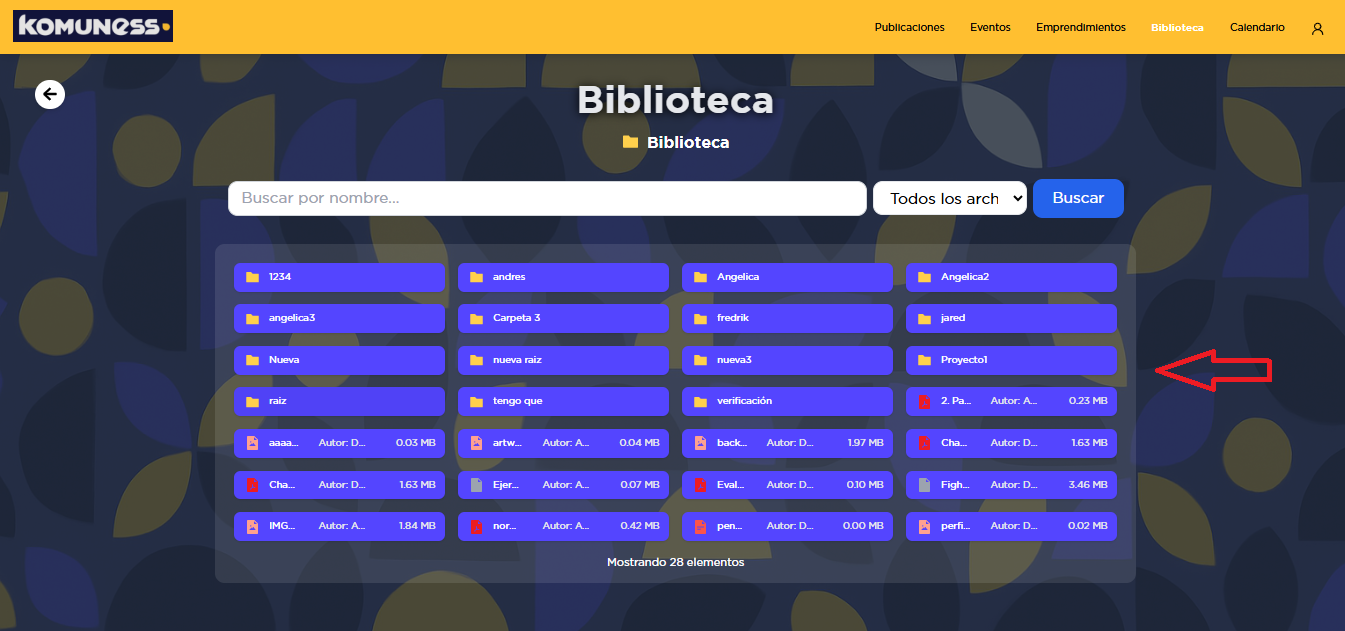
\includegraphics[width=\textwidth]{project/images/6.10.png}
  \caption{Vista optimizada de biblioteca digital con sistema de carpetas mejorado}
  \label{fig:biblio-vista}
\end{figure}


\begin{figure}[H]
  \centering
  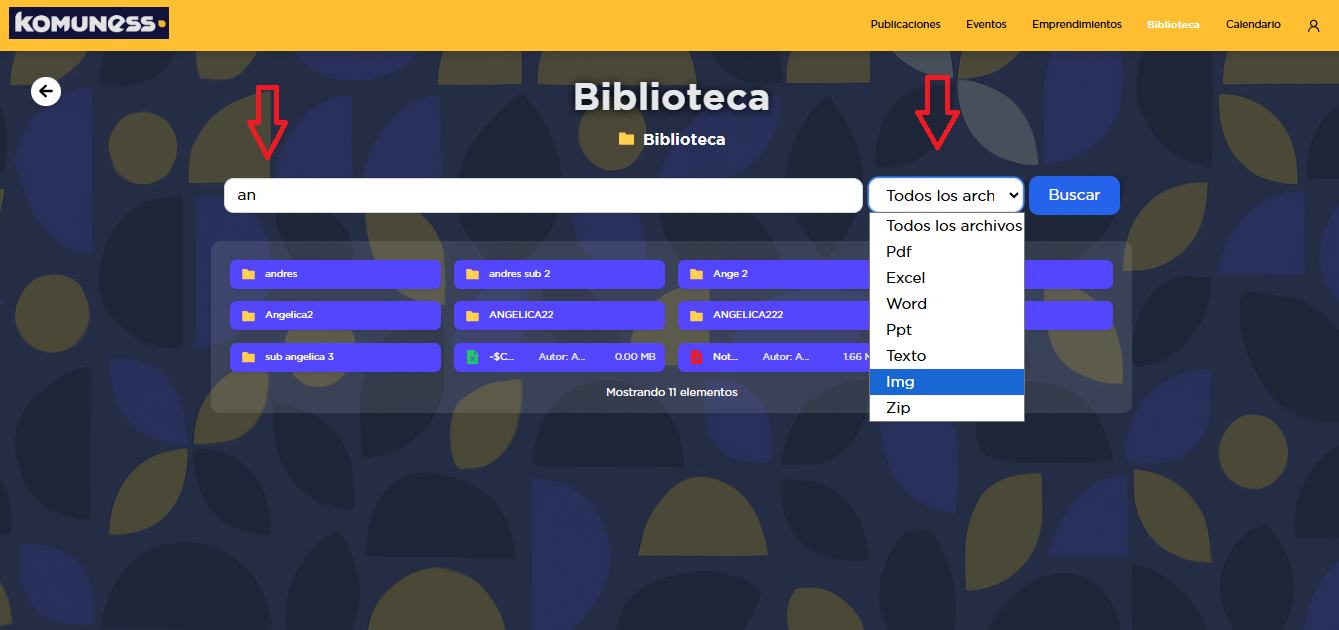
\includegraphics[width=\textwidth]{project/images/6.12}
  \caption{Filtros de búsqueda mejorados en biblioteca digital}
  \label{fig:biblio-filtros}
\end{figure}

\section{Capturas de Adaptación Responsive}

\begin{figure}[H]
  \centering
  % Opción 1: ancho fijo en centímetros
  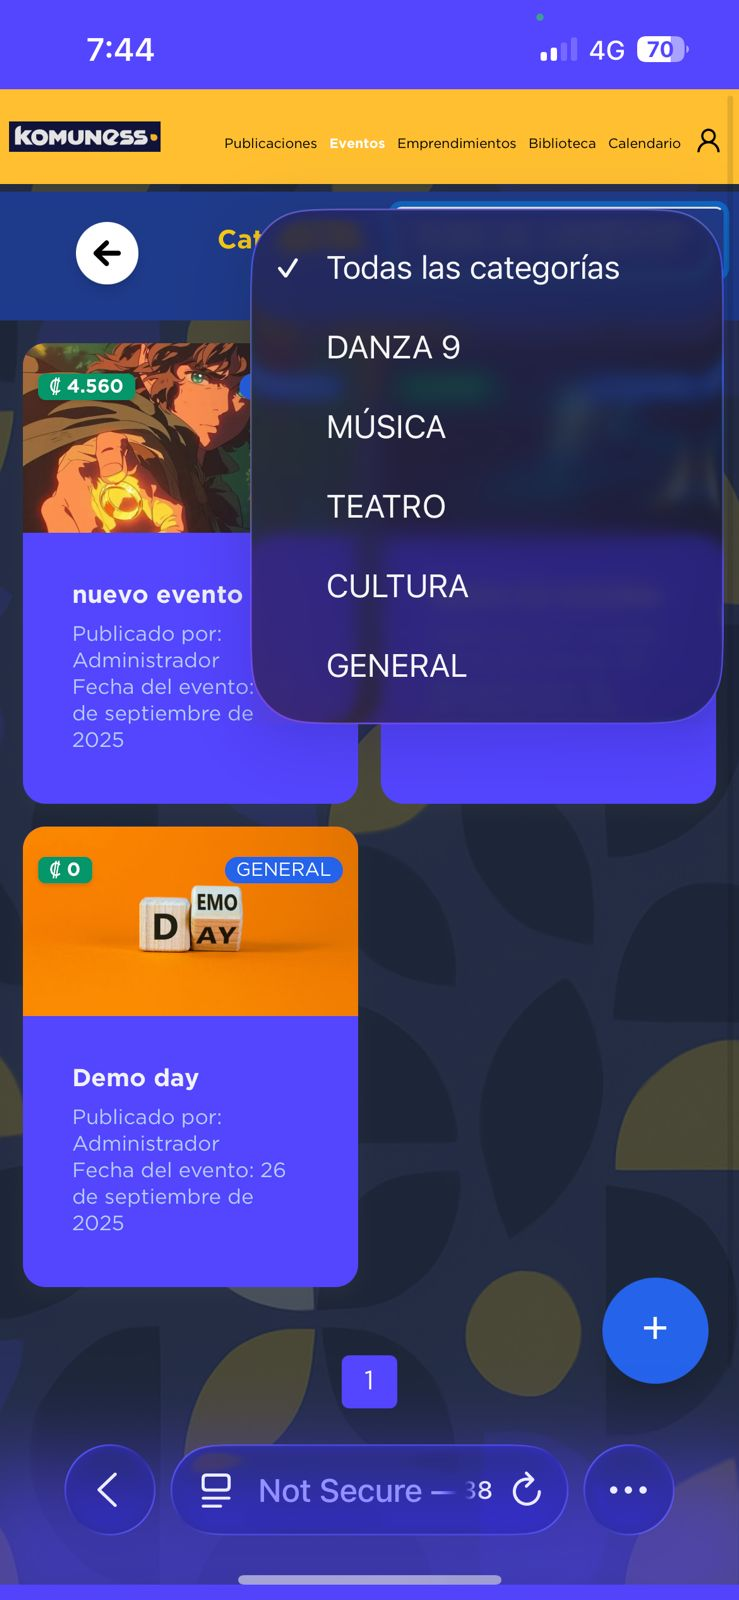
\includegraphics[width=4cm,keepaspectratio]{project/images/imagen13.jpg}
  \caption{Vista móvil del sistema de categorías adaptada para pantallas pequeñas}
  \label{fig:resp-movil}
\end{figure}

\begin{figure}[H]
  \centering
  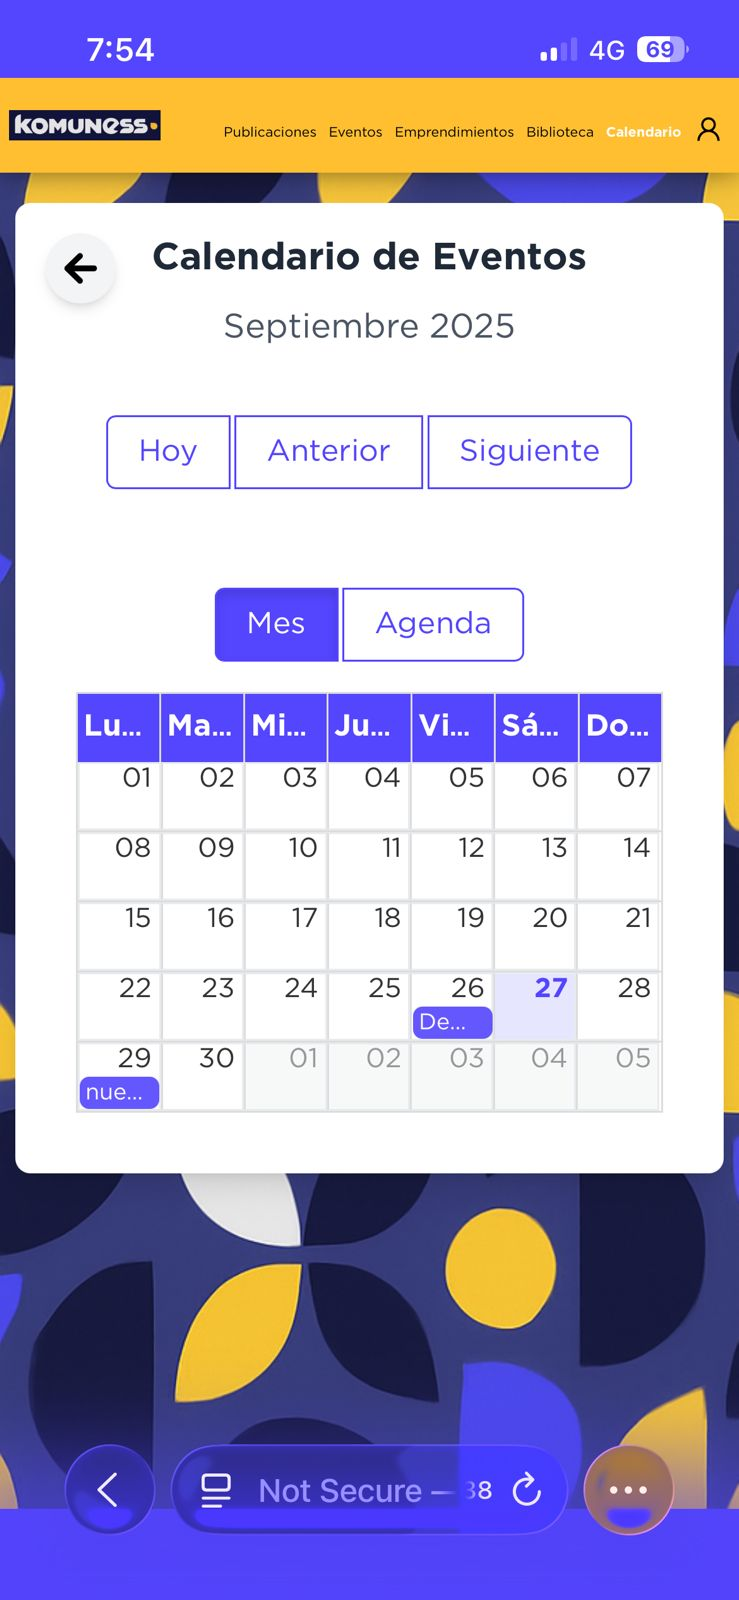
\includegraphics[width=4cm,keepaspectratio]{project/images/imagen14.jpg}
  \caption{Calendario interactivo en dispositivo movil}
  \label{fig:resp-tablet}
\end{figure}

\section{Capturas de Correcciones Frontend}

\begin{figure}[H]
  \centering
  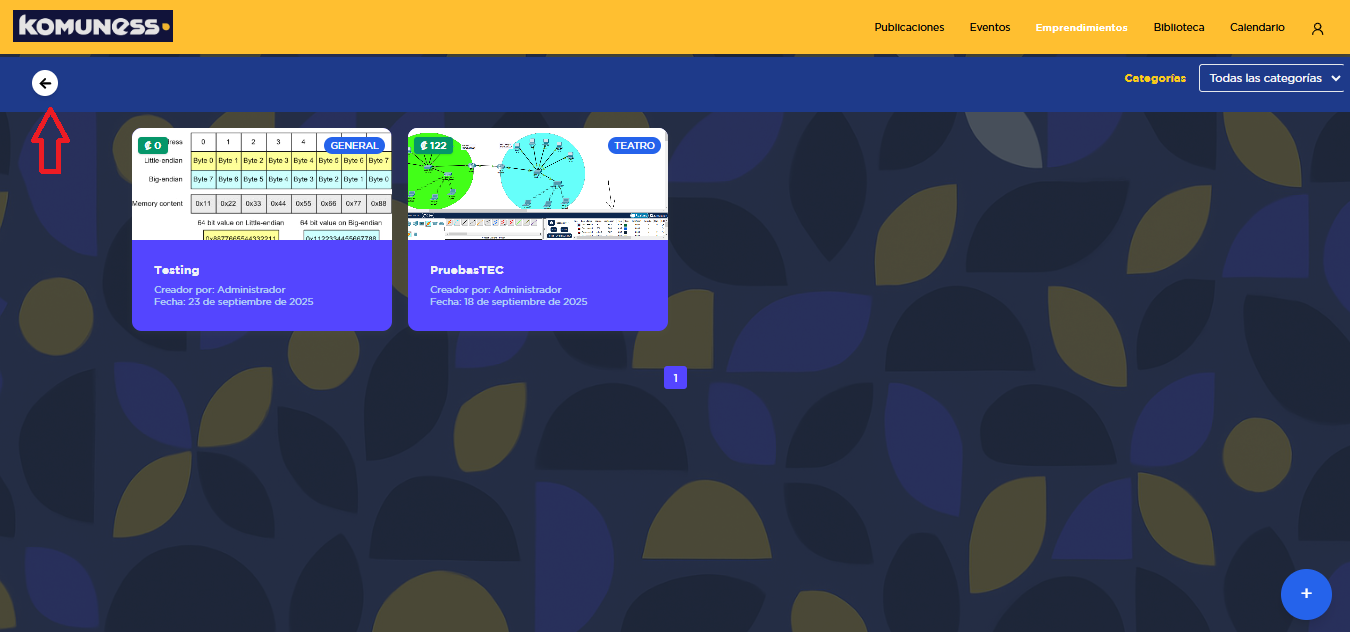
\includegraphics[width=\textwidth]{project/images/6.13.png}
  \caption{Vista de apartados con elementos corregidos y botones ``Volver'' implementados}
  \label{fig:frontend-navegacion}
\end{figure}

\begin{figure}[H]
  \centering
  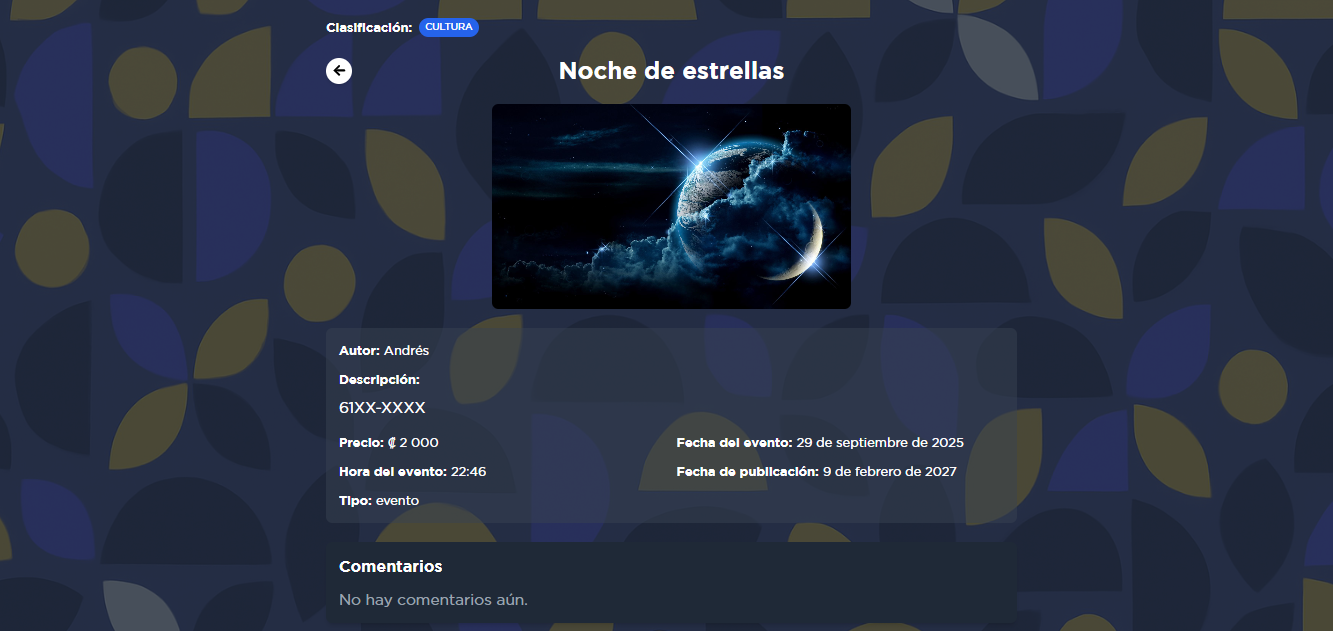
\includegraphics[width=\textwidth]{project/images/6.15.png}
  \caption{Cards de publicaciones con información completa y precio visible}
  \label{fig:frontend-cards}
\end{figure}
 % [OPCIONAL] Capturas de pantalla
\chapter{Conclusiones y trabajo futuro}

\section{Conclusiones}
El Sprint 1 del proyecto \textbf{Komuness} ha resultado en la entrega exitosa de un MVP estable y funcional que establece bases sólidas para el desarrollo futuro de la plataforma comunitaria. Los principales logros alcanzados demuestran la viabilidad técnica del sistema y su potencial impacto en la comunidad de Tejarcillos, Alajuelita.

Entre los logros más relevantes se destacan:

\begin{itemize}
    \item \textbf{Implementación del sistema de categorías:} Se desarrolló un sistema robusto de clasificación temática que mejora significativamente la organización del contenido. Los usuarios pueden filtrar publicaciones por áreas específicas (arte, cultura, deporte, educación), lo que facilita el descubrimiento de información relevante. Incluye interfaces administrativas completas y herramientas de usuario intuitivas, constituyendo un modelo escalable para futuras expansiones.
    
    \item \textbf{Calendario interactivo funcional:} Se implementó un calendario que permite visualizar y gestionar eventos comunitarios. La integración fluida con el sistema de publicaciones y campos específicos para eventos (precio y hora) genera un ecosistema cohesivo que fortalece la participación comunitaria.
    
    \item \textbf{Estabilización y optimización del sistema base:} Las correcciones en frontend y backend transformaron un sistema parcialmente funcional en una plataforma estable. Las mejoras en navegación, visualización, adaptación responsive y manejo de errores elevaron significativamente la experiencia de usuario.
    
    \item \textbf{Fortalecimiento del sistema de archivos:} Se optimizó la biblioteca digital mediante estrategias híbridas de almacenamiento (nube para imágenes y local para documentos), logrando un sistema robusto y económicamente viable para la gestión de recursos multimedia.
    
    \item \textbf{Validación de la arquitectura MERN:} El stack tecnológico seleccionado demostró ser adecuado para aplicaciones comunitarias, al ofrecer flexibilidad, escalabilidad y facilidad de mantenimiento. La separación entre frontend y backend facilita el desarrollo paralelo y futuras expansiones.
    
    \item \textbf{Metodología de desarrollo efectiva:} El uso de prácticas SCRUM, control de versiones con Git y testing automatizado resultó en un proceso de desarrollo organizado y predecible. La velocidad del equipo de 21 puntos establece una línea base realista para futuras iteraciones.
\end{itemize}

\section{Problemáticas y limitaciones}
El sistema presenta las siguientes problemáticas y limitaciones:

\subsection*{Problemáticas}
\begin{itemize}
     \item \textbf{Dependencias de infraestructura externa:} El uso de servicios como Digital Ocean Spaces y MongoDB Atlas puede generar costos operativos y puntos de falla a considerar en la planificación a largo plazo (mongodb,2025).
    
    \item \textbf{Ausencia de sistema de notificaciones:} Actualmente no existen mecanismos para avisar sobre nuevas publicaciones, eventos próximos o comentarios, lo cual limita el engagement comunitario.
    \item \textbf{Funcionalidad de búsqueda básica:} El sistema no implementa búsqueda de texto completo ni algoritmos de relevancia, restringiendo la experiencia de descubrimiento de contenido (fielding,2000).
    \item \textbf{Limitaciones en moderación de contenido:} La plataforma depende únicamente de la intervención manual, careciendo de herramientas automatizadas para detección o workflows de aprobación.
\end{itemize}

\subsection*{Limitaciones}
\begin{itemize}
    \item \textbf{Escalabilidad en almacenamiento local:} La estrategia actual, aunque económica, puede volverse insuficiente a medida que aumente el volumen de archivos, ya que no incluye compresión ni archivado automático.
    \item \textbf{Plataformas soportadas:} El sistema está optimizado para navegadores modernos (Chrome 90+, Firefox 88+, Safari 14+, Edge 90+). La funcionalidad puede verse limitada en versiones anteriores. No existe aplicación móvil nativa, dependiendo del navegador móvil.
    \item \textbf{Requerimientos técnicos:} Se requiere conexión a internet estable, JavaScript habilitado y al menos 2GB de RAM libre en el dispositivo cliente. La experiencia se degrada en conexiones lentas (<1Mbps).
\end{itemize}

\section{Trabajo futuro}
Como líneas de mejora y expansión se proponen las siguientes iniciativas:

\begin{itemize}
    \item \textbf{Sistema de membresías premium y monetización (Sprint 2):} Integración con PayPal, creación de niveles de membresía con beneficios diferenciados y límites configurables en publicaciones, garantizando la sostenibilidad económica del proyecto.
    
    \item \textbf{Perfiles públicos y banco de profesionales (Sprint 2–3):} Desarrollo de perfiles detallados que permitan mostrar habilidades, experiencias y servicios. El banco de profesionales fomentará conexiones y el desarrollo económico local.
    
    \item \textbf{Sistema de notificaciones y engagement:} Implementación de notificaciones push web, correos automáticos para eventos próximos y herramientas de interacción como “me gusta” y compartir en redes sociales.
    
    \item \textbf{Mejoras en búsqueda y descubrimiento:} Desarrollo de búsqueda de texto completo, algoritmos de relevancia, filtros combinados y recomendaciones basadas en intereses y actividad del usuario.
    
    \item \textbf{Herramientas de moderación y administración:} Automatización de detección de contenido inapropiado, workflows de aprobación y paneles administrativos avanzados.
    
    \item \textbf{Optimización de performance:} Aplicación de lazy loading, caching estratégico, optimización de consultas a la base de datos y compresión de recursos para mejorar tiempos de carga en conexiones lentas.
    
    \item \textbf{Funcionalidades sociales avanzadas:} Desarrollo de mensajería privada, grupos temáticos, eventos recurrentes en calendario e integración con redes sociales externas.
    
    \item \textbf{Analítica y métricas:} Creación de un dashboard de analíticas para administradores con métricas de engagement, contenido popular, patrones de uso y crecimiento comunitario.
\end{itemize}
 % Conclusiones del informe


\bibliographystyle{apacite}
% Muestra TODAS las entradas del .bib aunque no estén citadas
\nocite{*}
\bibliography{project/references.bib}

\end{document}
